\documentclass[a4paper, 12pt]{article}

\usepackage[english,russian]{babel}
\usepackage[left=2cm, top=2cm, right=2cm, bottom=2.5cm]{geometry}
\usepackage{amssymb}
\usepackage{amsmath}
\usepackage{graphicx}
\usepackage[tableposition=top,singlelinecheck=false]{caption}

\title{Измерение теплоёмкости железного и алюминиевого конусов. Оценка точности измерений.}
\author{Леонид Пилюгин, Б02-212}

\begin{document}
    \maketitle

    \section{Параметры установки и исследуемых тел}

    \begin{enumerate}
        \item Масса железного цилиндра $m_\text{Fe}=815{,}1\pm 0{,}1\,\text{г}$
        \item Масса алюминиевого цилиндра $m_\text{Fe}=294{,}2\pm 0{,}1\,\text{г}$
        \item Зависимость темепратуры калориметра от измеряемого сопротивления:
        \[T=14{,}377980252039598845\,\frac{^\circ\text{C}}{\text{Ом}}\cdot R + 39{,}35514018691588785\,^\circ\text{C} - 273\,^\circ\text{C}\]
        \item Напряжение нагревателя $U=26{,}6502\pm0{,}0005\,\text{В}$
        \item Ток нагревателя $I=223{,}4\pm0{,}05\,\text{мА}$
    \end{enumerate}

    \section{Измеряемые данные}
    \begin{figure}[ht!]
        \centering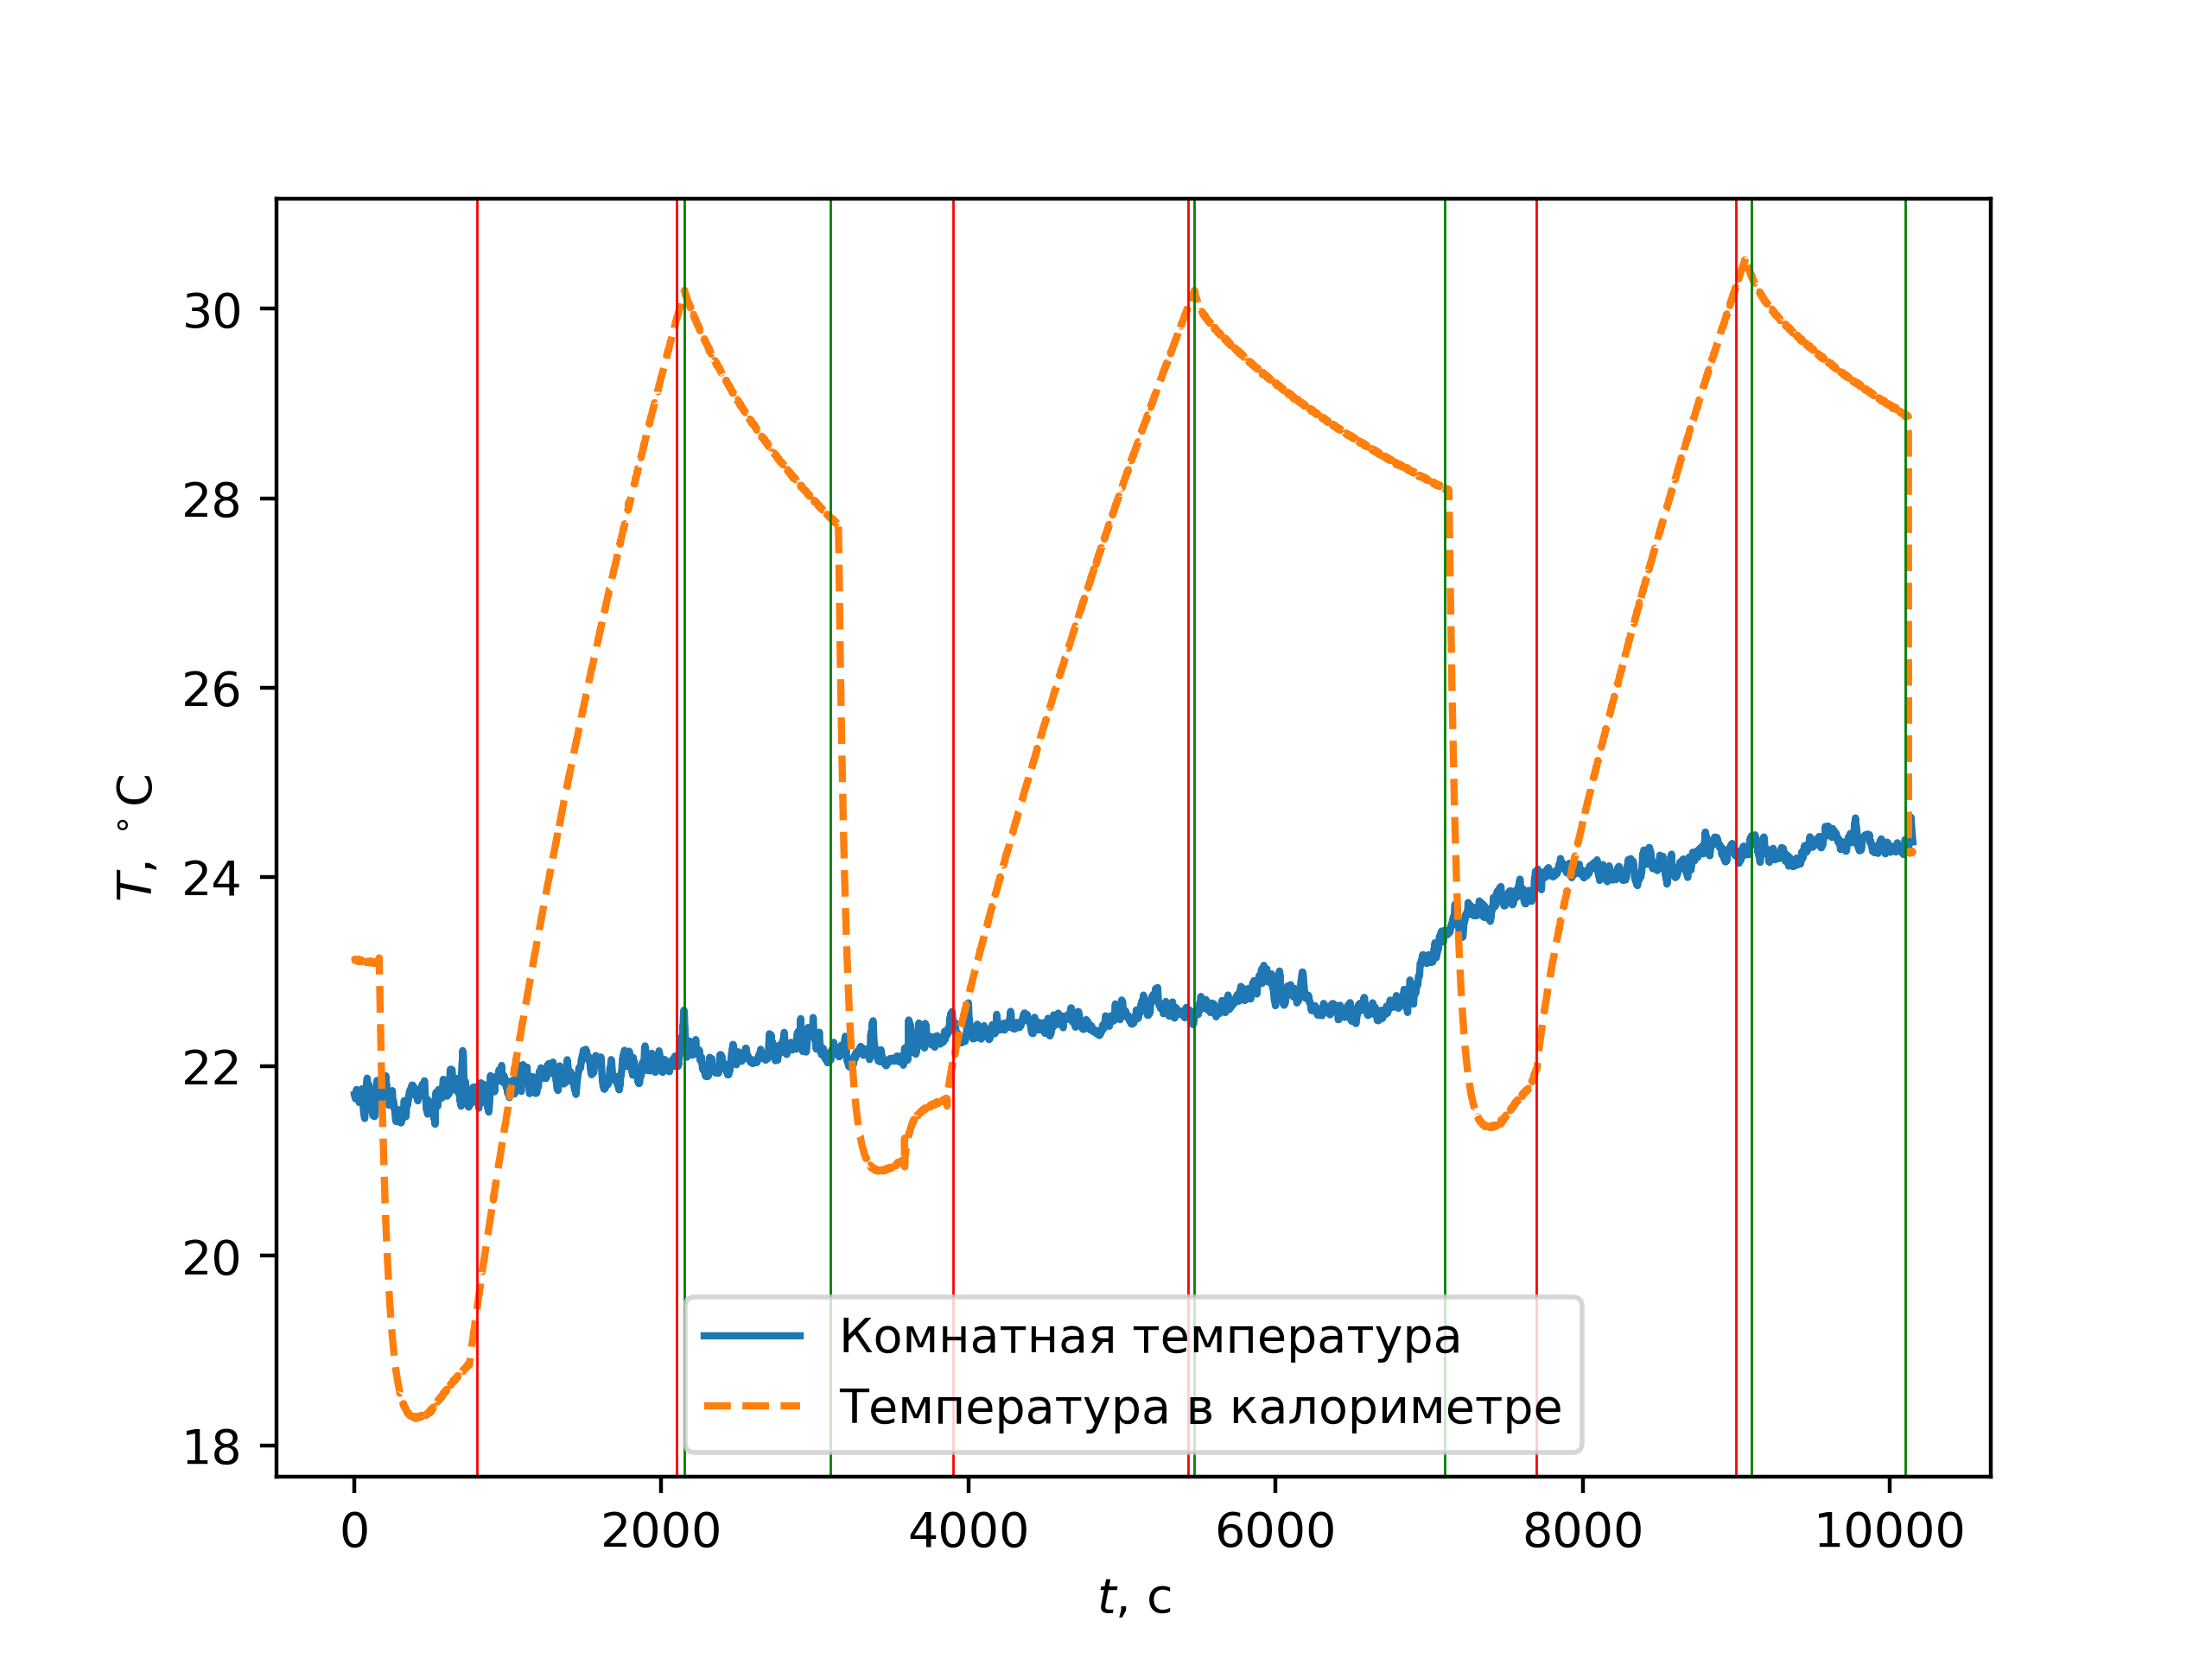
\includegraphics[width=0.8\linewidth]{img/fig.png}
        \caption{Кривые температур в калориметре и снаружи}
    \end{figure}

    Измереныые кривые температур снаружи и внутри калориметра (для удобства представления
    сопротивление пересчитано в температуру).
    Между красными вертикальными линиями расположены интервалы нагревания, зелёными~--- охлаждения.

    Этим чертам слева направо соответствуют моменты времени $800\,\text{с}$,  $2100\,\text{с}$,
    $2150\,\text{с}$, $3100\,\text{с}$, $3900\,\text{с}$, $5430\,\text{с}$, $5470\,\text{с}$,
    $7100\,\text{с}$, $7700\,\text{с}$, $9000\,\text{с}$, $9100\,\text{с}$, $10100\,\text{с}$.

    \section{Обработка данных}
    \subsection{Интегральный метод}
    В этом методе используется предположение, что комнатная температура примено постоянна
    на протяжении измерений.

    Тогда температура остывающего калориметра $T_\text{cool}$ связана со временем $t$
    соотношением
    \[T_\text{cool}=(T-T_\text{K})\exp\left(-\frac{\lambda}{C}t\right)+t_\text{K}\]
    $T$~--- температура в начале охлаждения, $T_\text{K}$~--- средняя комнатная температура,
    $\lambda$~--- коэффициент теплопроводности калориметра и его содержимого, $C$~--- теплоёмкость  калориметра и его содержимого.

    Построив зависимость температуры охлаждающегося калориметра от времени в координатах
    $\left(\ln\frac{T_\text{cool}-T_\text{K}}{T-T_\text{K}},t\right)$ получим прямую,
    наклон которой равен $-\frac{C}{\lambda}$.

    При нагревании с мощностью $P$ температура калориметра $T_\text{heat}$ зависит от 
    времени $t$ следующим образом:
    \[T_\text{heat}=\frac{P}{\lambda}\left(1-\exp\left(-\frac{\lambda}{C}t\right)\right)+T_\text{K}\]
    $T$~--- температура в начале нагревания, $T_\text{K}$~--- средняя комнатная температура,
    $\lambda$~--- коэффициент теплопроводности калориметра и его содержимого, $C$~--- теплоёмкость  калориметра и его содержимого.

    Построив эту зависимость в координатах $\left(P\left(1-\exp\left(-\frac{\lambda}{C}t\right)\right), T-T_\text{K}\right)$,
    получаем прямую с наклоном $\lambda$.

    Мощность $P$ вычисляется через ток и напряжение нагревателя. $$P=UI=5{.}9430\pm0{,}0014\,\text{Вт}$$.

    \subsubsection{Определение теплоёмкости пустого калориметра}
    Построив кривую охлаждения в интервале времени $(2650;\;3100)\,\text{с}$,
    получаем $$\frac{C}{\lambda}=3129\pm 4\,\text{с}$$.
    \begin{figure}[ht!]
        \centering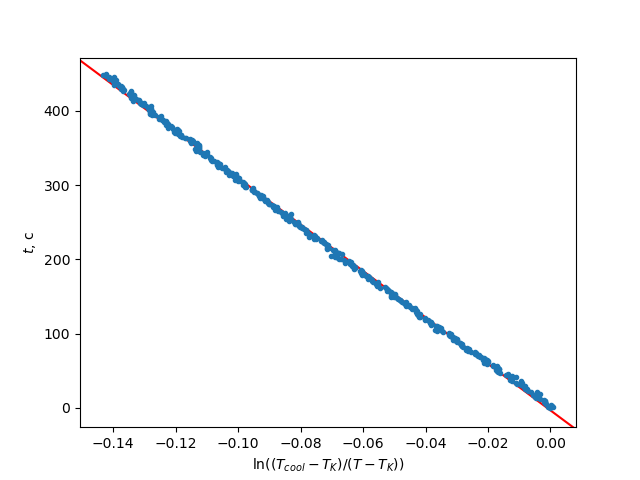
\includegraphics[width=0.6\linewidth]{img/lce.png}
        \caption{Кривая охлаждения пустого калориметра}
    \end{figure}

    Построив кривую нагревания в интервале $(1100;\;2100)\,\text{с}$, получаем
    $$\lambda=0{,}22133\pm 0{,}00010\,\frac{\text{Вт}}{\text{К}}$$

    Тогда $$C=692{,}5\pm 1{,}3\,\frac{\text{Дж}}{\text{К}}$$

    \begin{figure}[ht!]
        \centering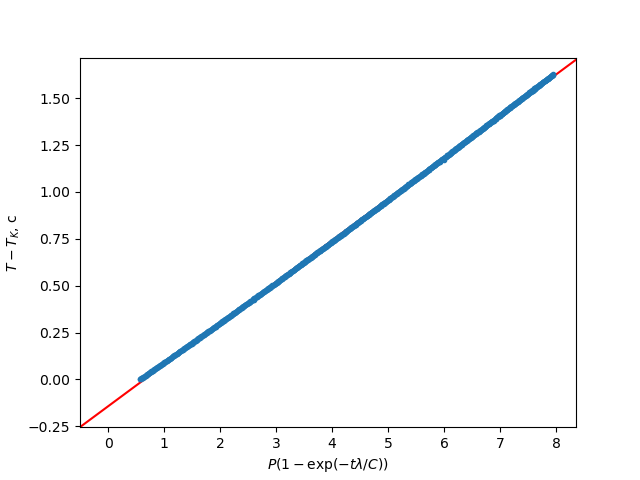
\includegraphics[width=0.6\linewidth]{img/lhe.png}
        \caption{Кривая нагревания пустого калориметра}
    \end{figure}

    \subsubsection{Определение теплоёмкости железа}
    Сначала определим теплоёмкость калориметра с железом.
    Построив кривую охлаждения в интервале времени $(5970;\;6900)\,\text{с}$,
    получаем $$\frac{C}{\lambda}=5776\pm 7\,\text{с}$$.

    \begin{figure}[ht!]
        \centering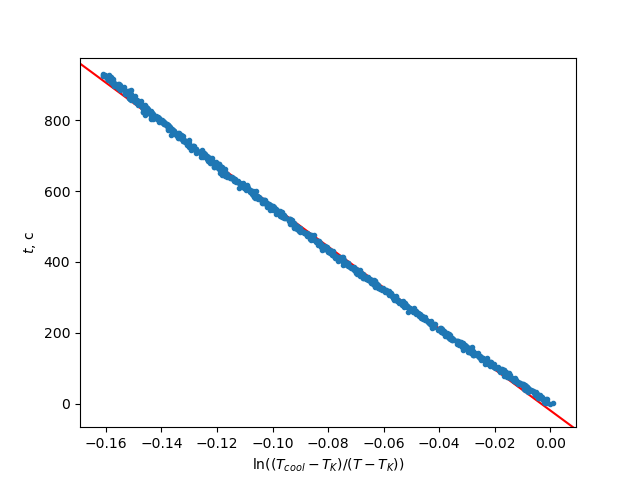
\includegraphics[width=0.6\linewidth]{img/lcf.png}
        \caption{Кривая охлаждения калориметра с железным цилиндром}
    \end{figure}

    Построив кривую нагревания в интервале $(4100;\;5430)\,\text{с}$, получаем
    $$\lambda=0{,}18484\pm 0{,}00008\,\frac{\text{Вт}}{\text{К}}$$

    Тогда $$C_\text{Fe}=1067{,}7\pm 1{,}8\,\frac{\text{Дж}}{\text{К}}$$
    $$c_\text{Fe}=\frac{C_\text{Fe}-C}{m_\text{Fe}}=460\pm 2\,\frac{\text{Дж}}{\text{кг}\cdot\text{К}}$$

    \begin{figure}[ht!]
        \centering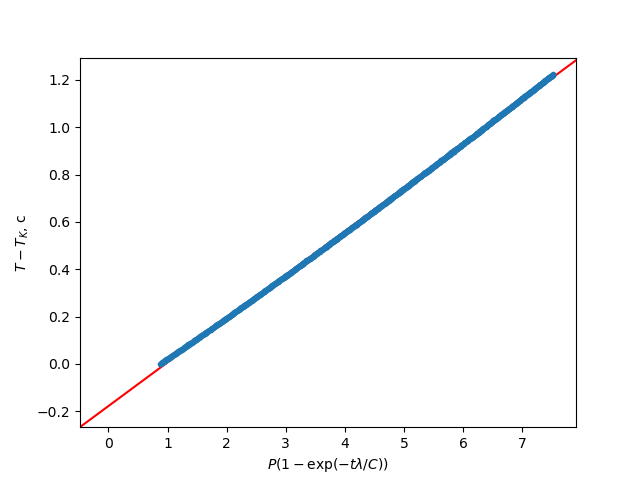
\includegraphics[width=0.6\linewidth]{img/lhf.png}
        \caption{Кривая нагревания с железным цилиндром}
    \end{figure}

    \subsubsection{Определение теплоёмкости алюминия}
    Сначала определим теплоёмкость калориметра с алюминием.
    Построив кривую охлаждения в интервале времени $(9600;\;10100)\,\text{с}$,
    получаем $$\frac{C}{\lambda}=4345\pm 8\,\text{с}$$.

    \begin{figure}[ht!]
        \centering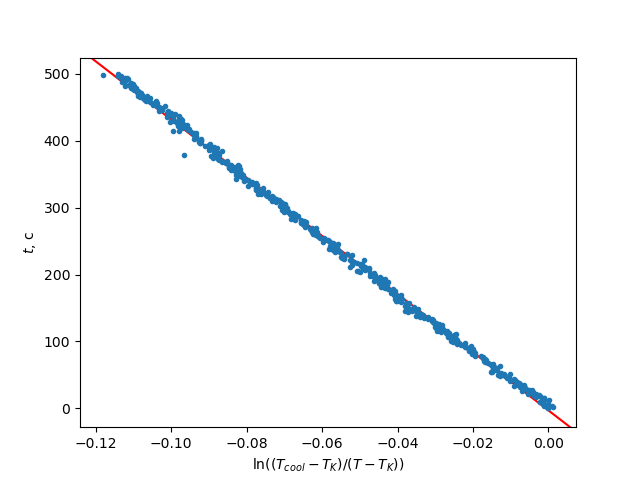
\includegraphics[width=0.6\linewidth]{img/lca.png}
        \caption{Кривая охлаждения калориметра с алюминиевым цилиндром}
    \end{figure}

    \begin{figure}[ht!]
        \centering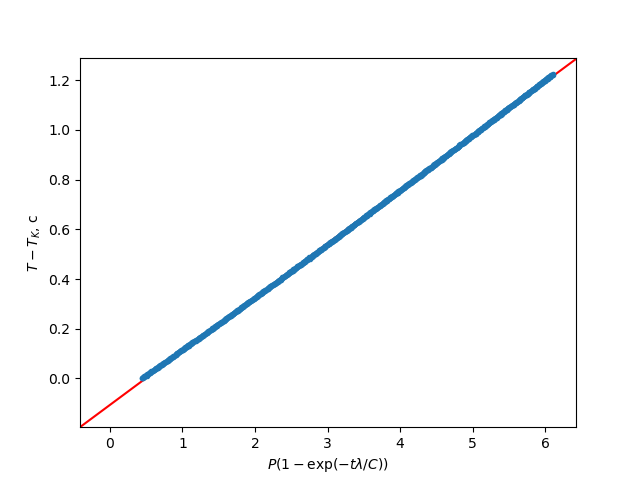
\includegraphics[width=0.6\linewidth]{img/lha.png}
        \caption{Кривая нагревания с алюминиевым цилиндром}
    \end{figure}

    Построив кривую нагревания в интервале $(8000;\;9000)\,\text{с}$, получаем
    $$\lambda=0{,}21670\pm 0{,}00009\,\frac{\text{Вт}}{\text{К}}$$

    Тогда $$C_\text{Al}=942{,}7\pm 2\,\frac{\text{Дж}}{\text{К}}$$
    $$c_\text{Al}=\frac{C_\text{Al}-C}{m_\text{Al}}=847\pm 2\,\frac{\text{Дж}}{\text{кг}\cdot\text{К}}$$

    Значения немного отличаются от табличных (450 и 920), что связано с изменением
    комнатной температуре в процессе эксперимента.


    \subsection{Дифференциальный метод в окрестности точек с комнатной температурой}
    В окрестности точек, где температура калориметра примерно равна комнатной,
    отсутсвтвуют теплопотери и вся мощность идёт на нагрев калориметра, т.е.
    \[C=\frac{P}{dT_\text{heat}/dt}\]
    
    Моменты совпадения температур при нагревании: $1013\,\text{с}$ (пустой),
    $3937\,\text{с}$ (с железным конусом), $7930\,\text{с}$ (с алюминиевым конусом).

    Наклоны графиков (оранжевые точки~--- значения комнатной температуры, синие~---
    температуры калориметра):
    \begin{enumerate}
        \item Пустой калориметр: $\frac{P}{C}=0{,}0010\pm 0{,}0003\,\text{К}/\text{с}$
        \item Калориметр с железом: $\frac{P}{C_\text{Fe}}=0{,}0070\pm 0{,}0002\,\text{К}/\text{с}$
        \item Калориметр с алюминием: $\frac{P}{C_\text{Al}}=0{,}0075\pm 0{,}0004\,\text{К}/\text{с}$
    \end{enumerate}

    \begin{gather*}
        C=598\pm16\,\frac{\text{Дж}}{\text{K}} \\
        C_\text{Fe}=850\pm20\,\frac{\text{Дж}}{\text{K}} \\
        C_\text{Al}=790\pm40\,\frac{\text{Дж}}{\text{K}} \\
        c_\text{Fe}=\frac{C-C_\text{Fe}}{m_\text{Fe}}=310\pm 30\,\frac{\text{Дж}}{\text{кг}\cdot\text{K}} \\
        c_\text{Al}=\frac{C-C_\text{Al}}{m_\text{Al}}=660\pm 150\,\frac{\text{Дж}}{\text{кг}\cdot\text{K}}
    \end{gather*}

    \begin{figure}[ht!]
        \centering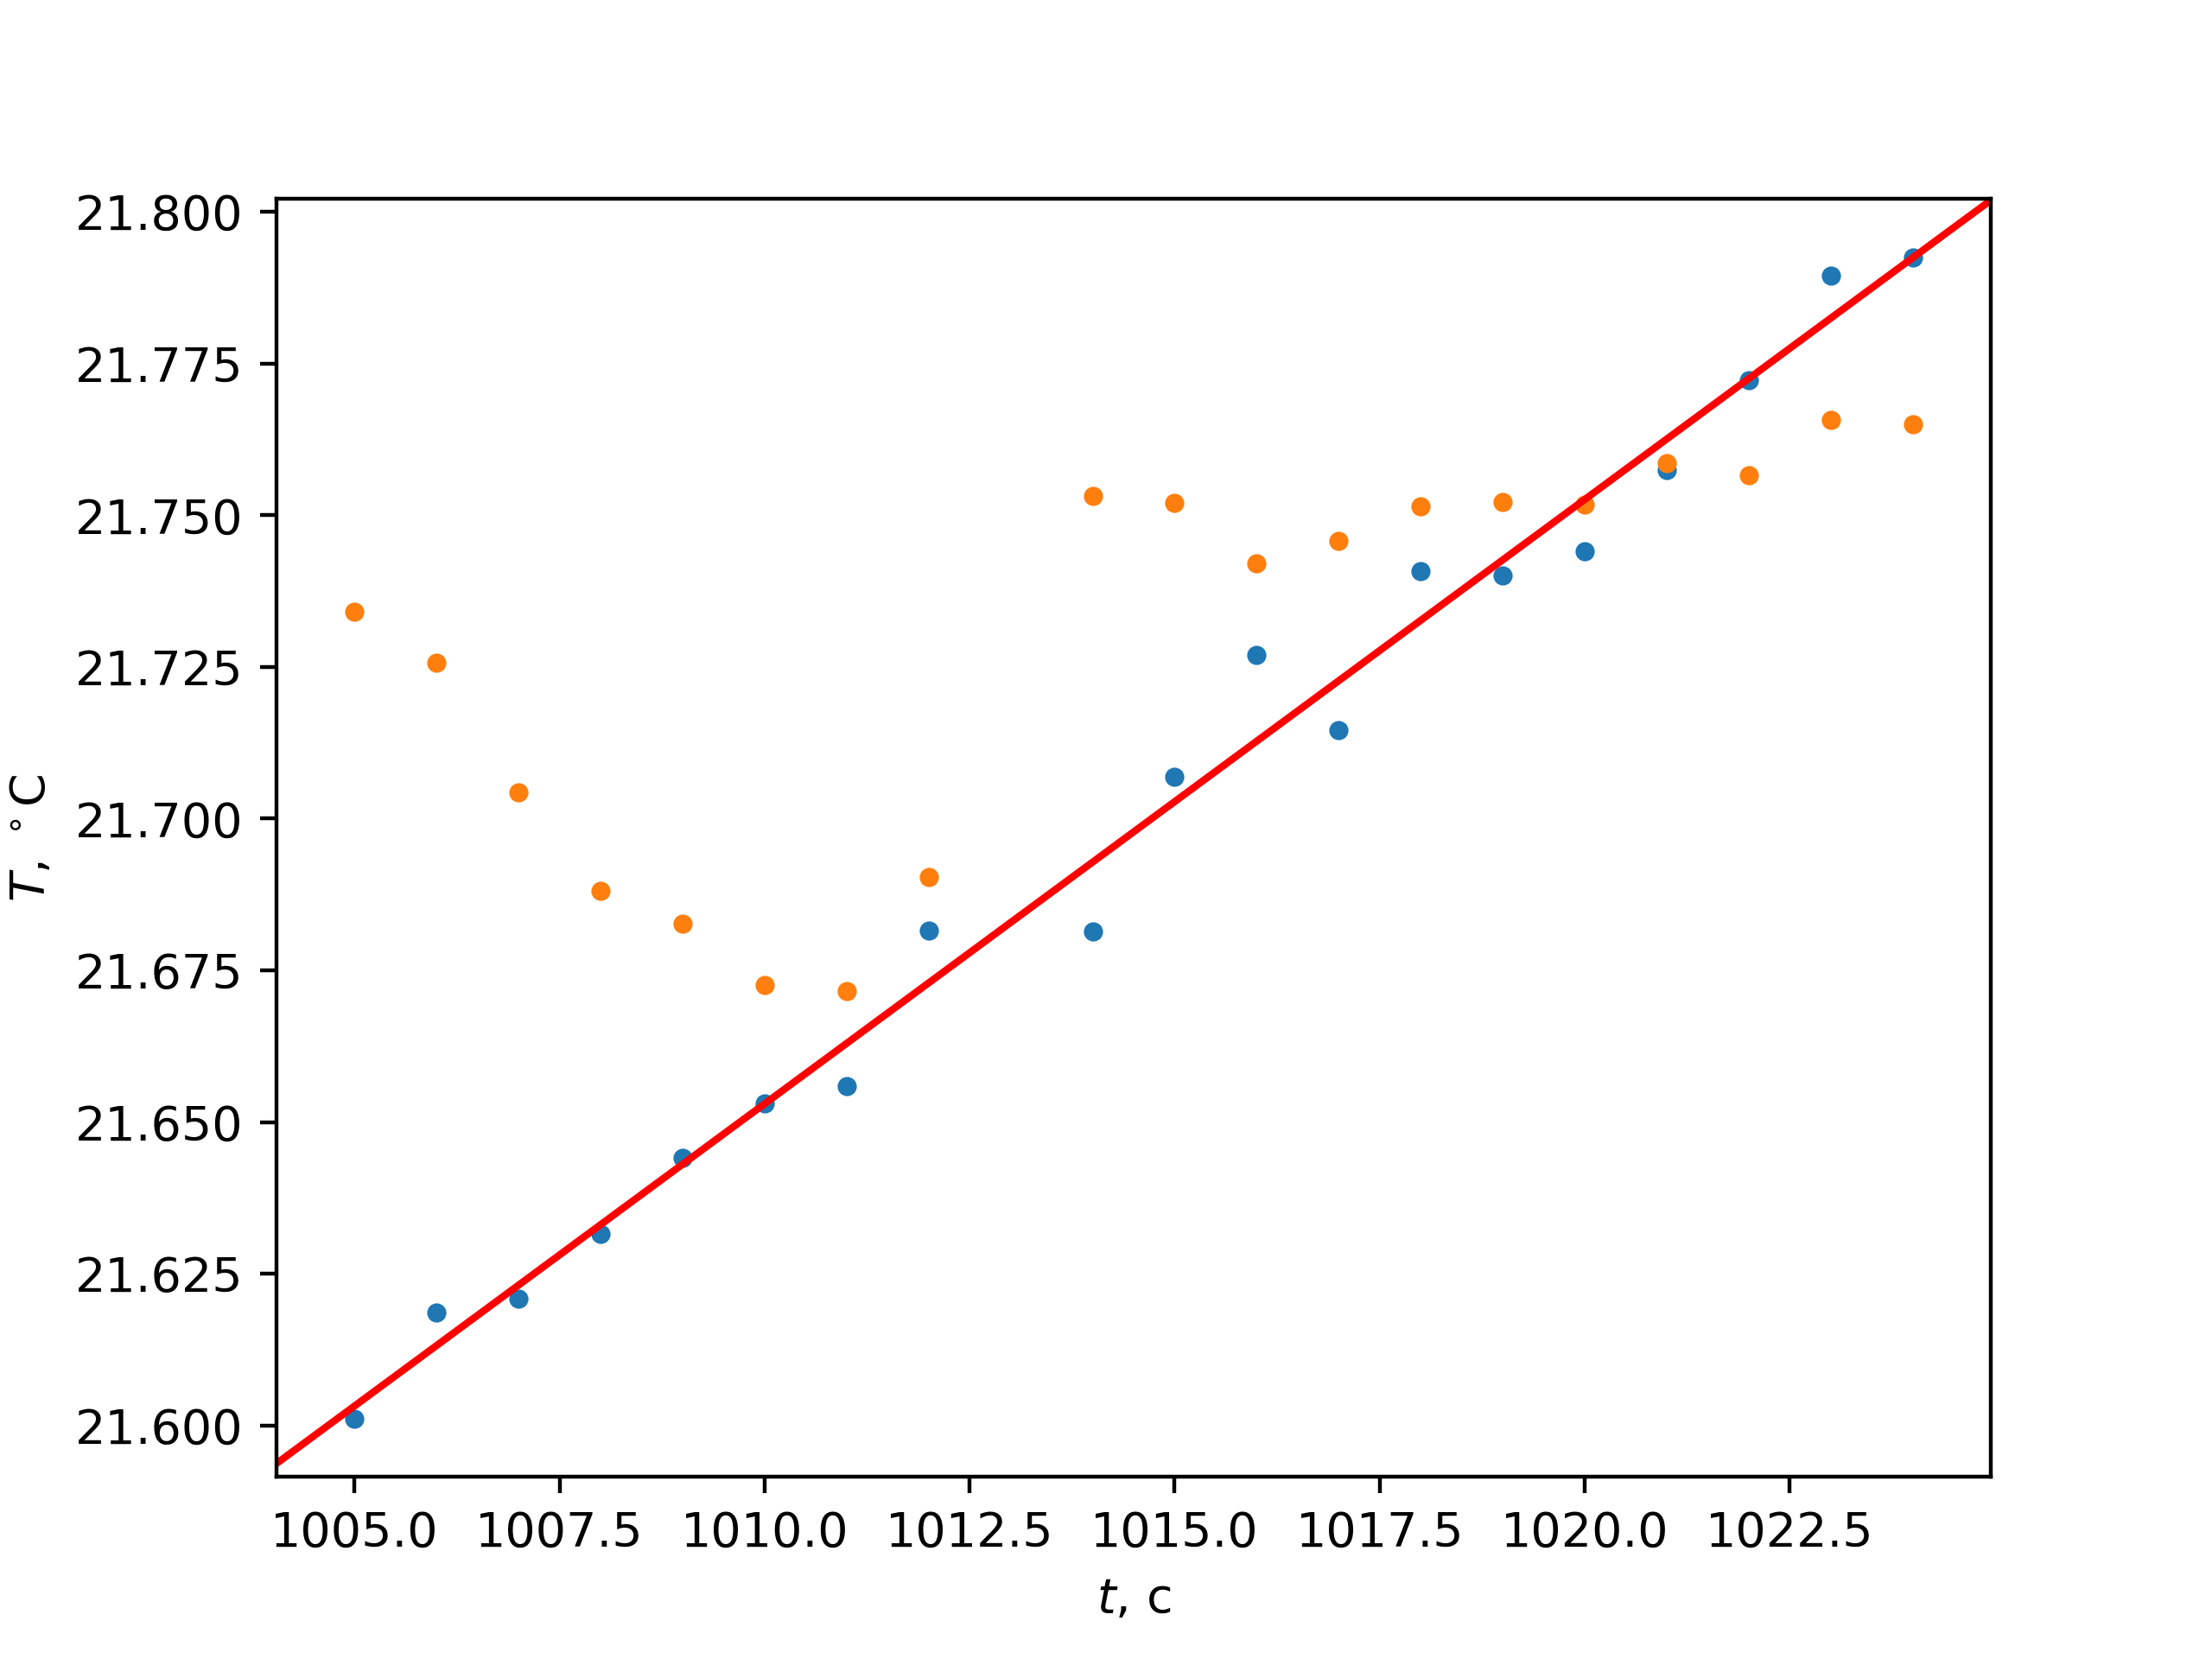
\includegraphics[width=0.6\linewidth]{img/1013.png}
        \caption{Касательная к кривой нагрева пустого калориметра}
    \end{figure}
    \begin{figure}[ht!]
        \centering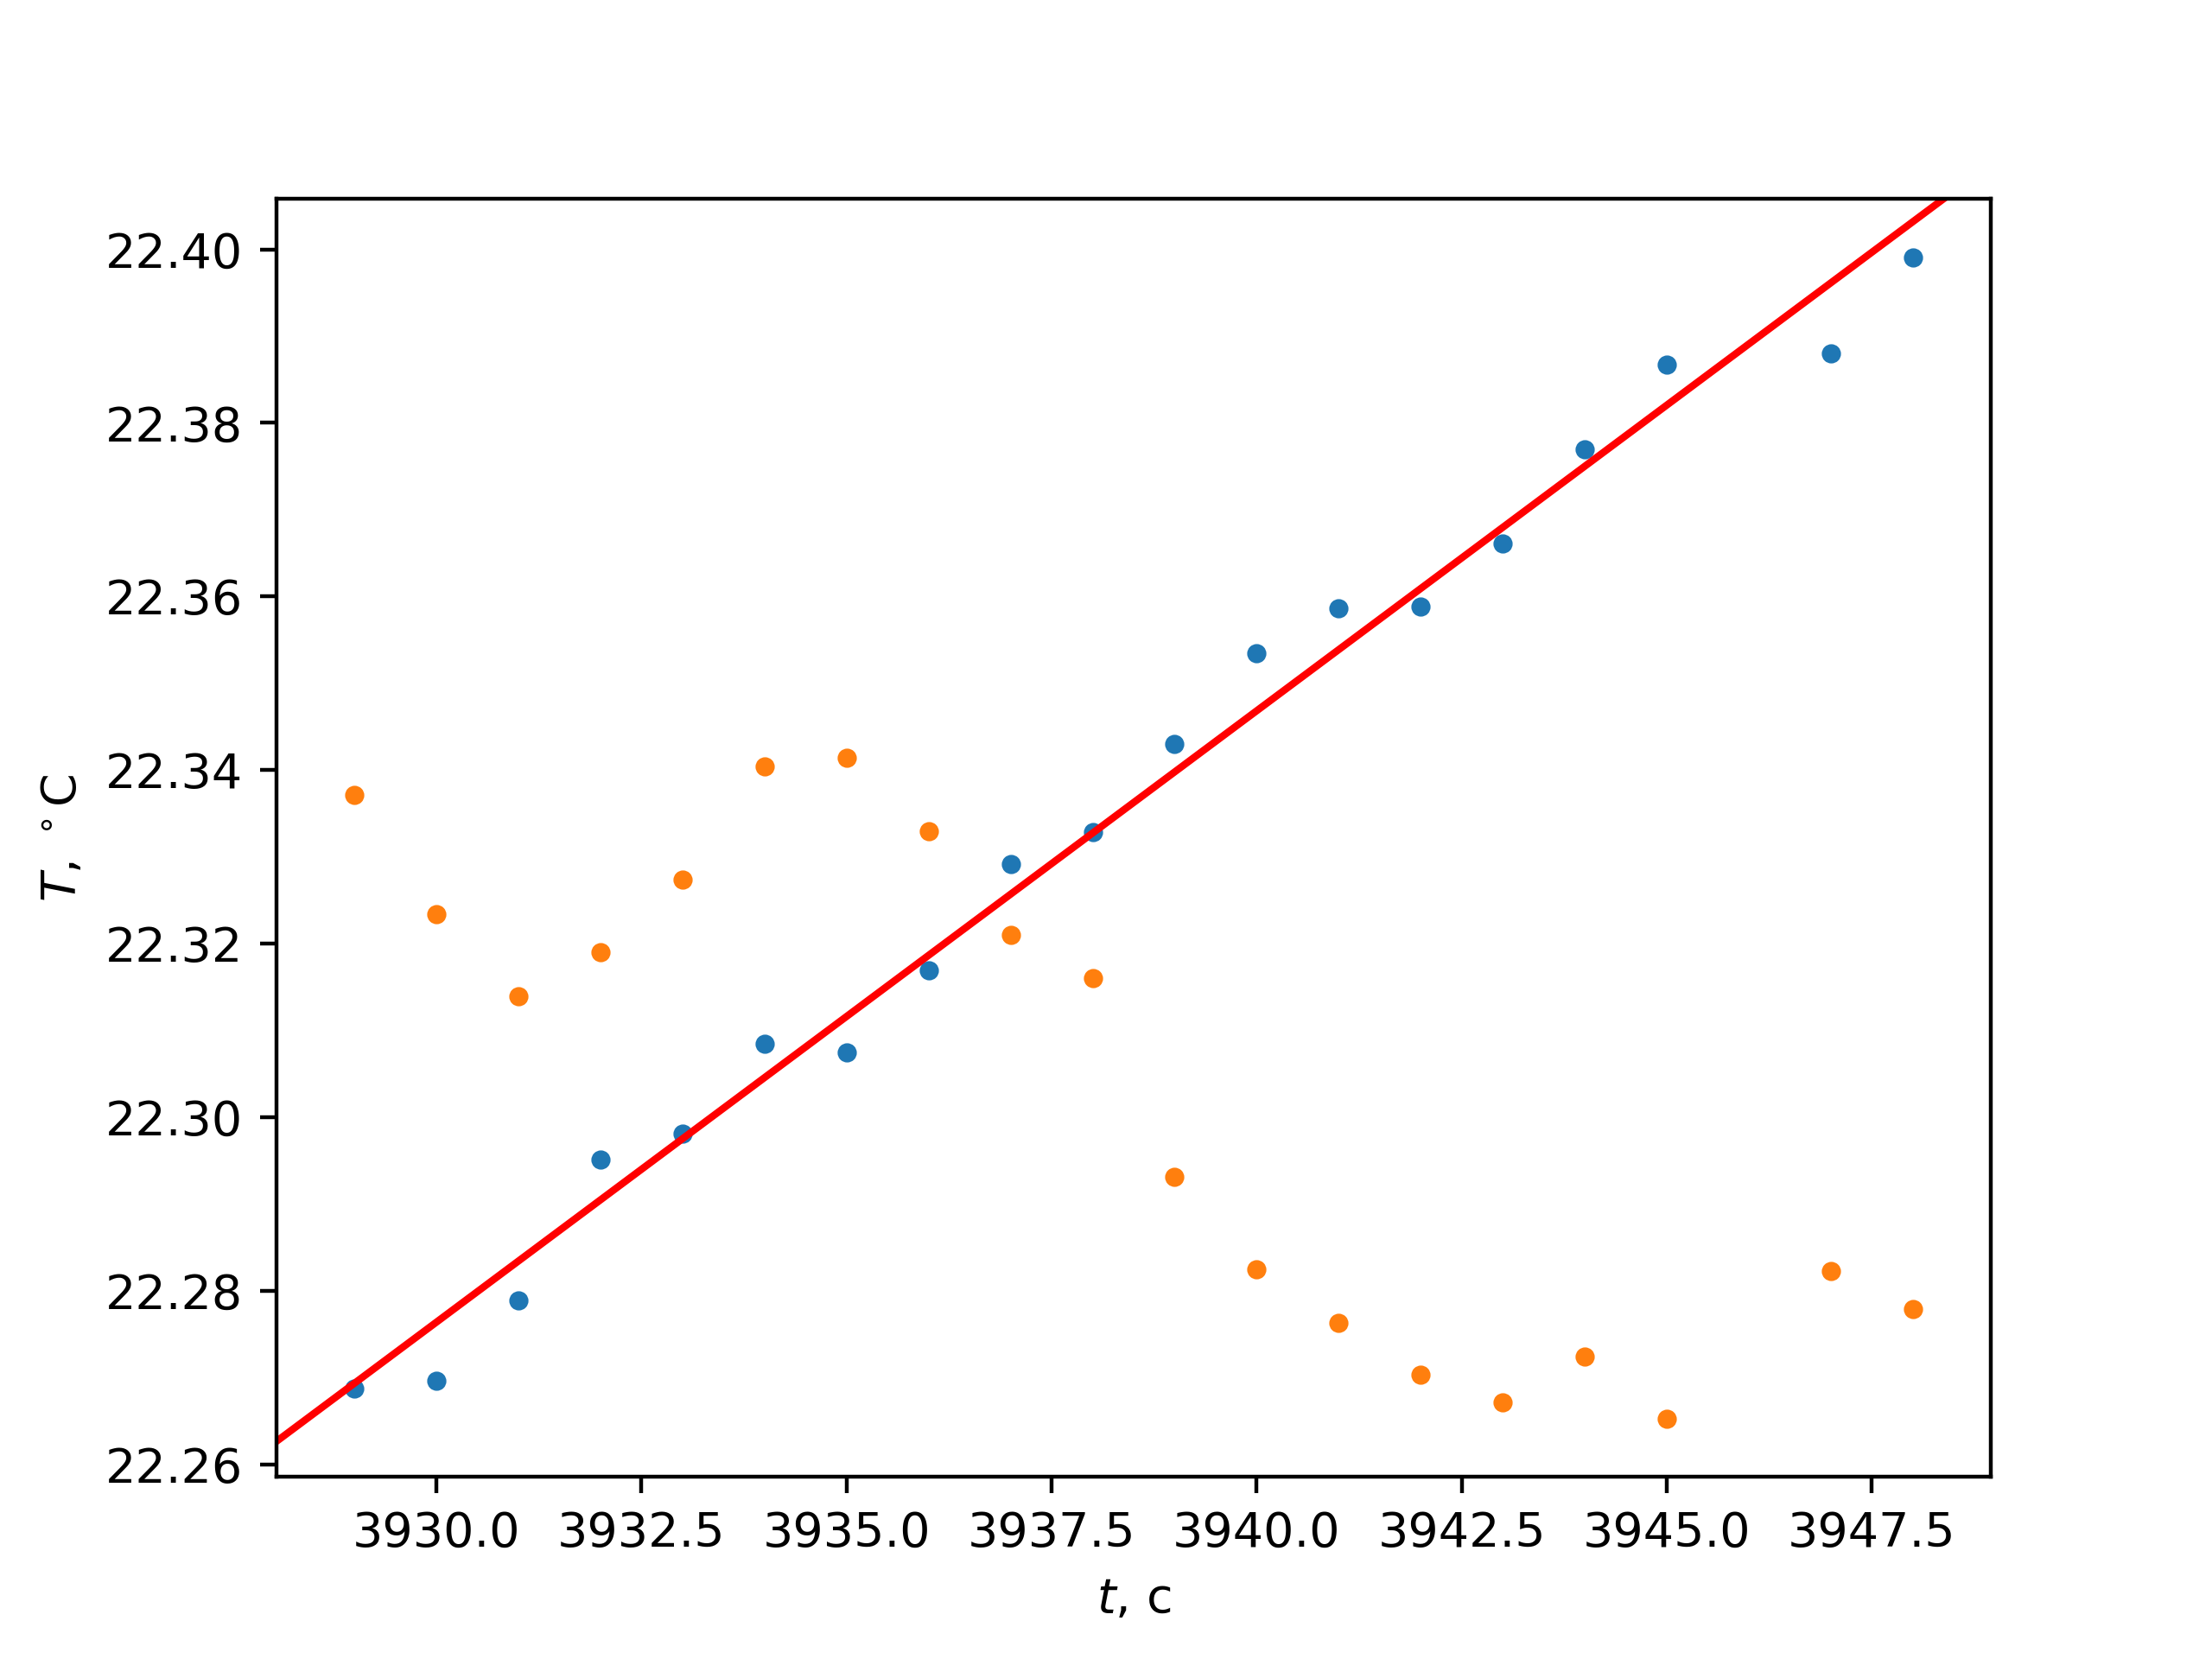
\includegraphics[width=0.6\linewidth]{img/3937.png}
        \caption{Касательная к кривой нагрева калориметра с железным конусом}
    \end{figure}
    \begin{figure}[ht!]
        \centering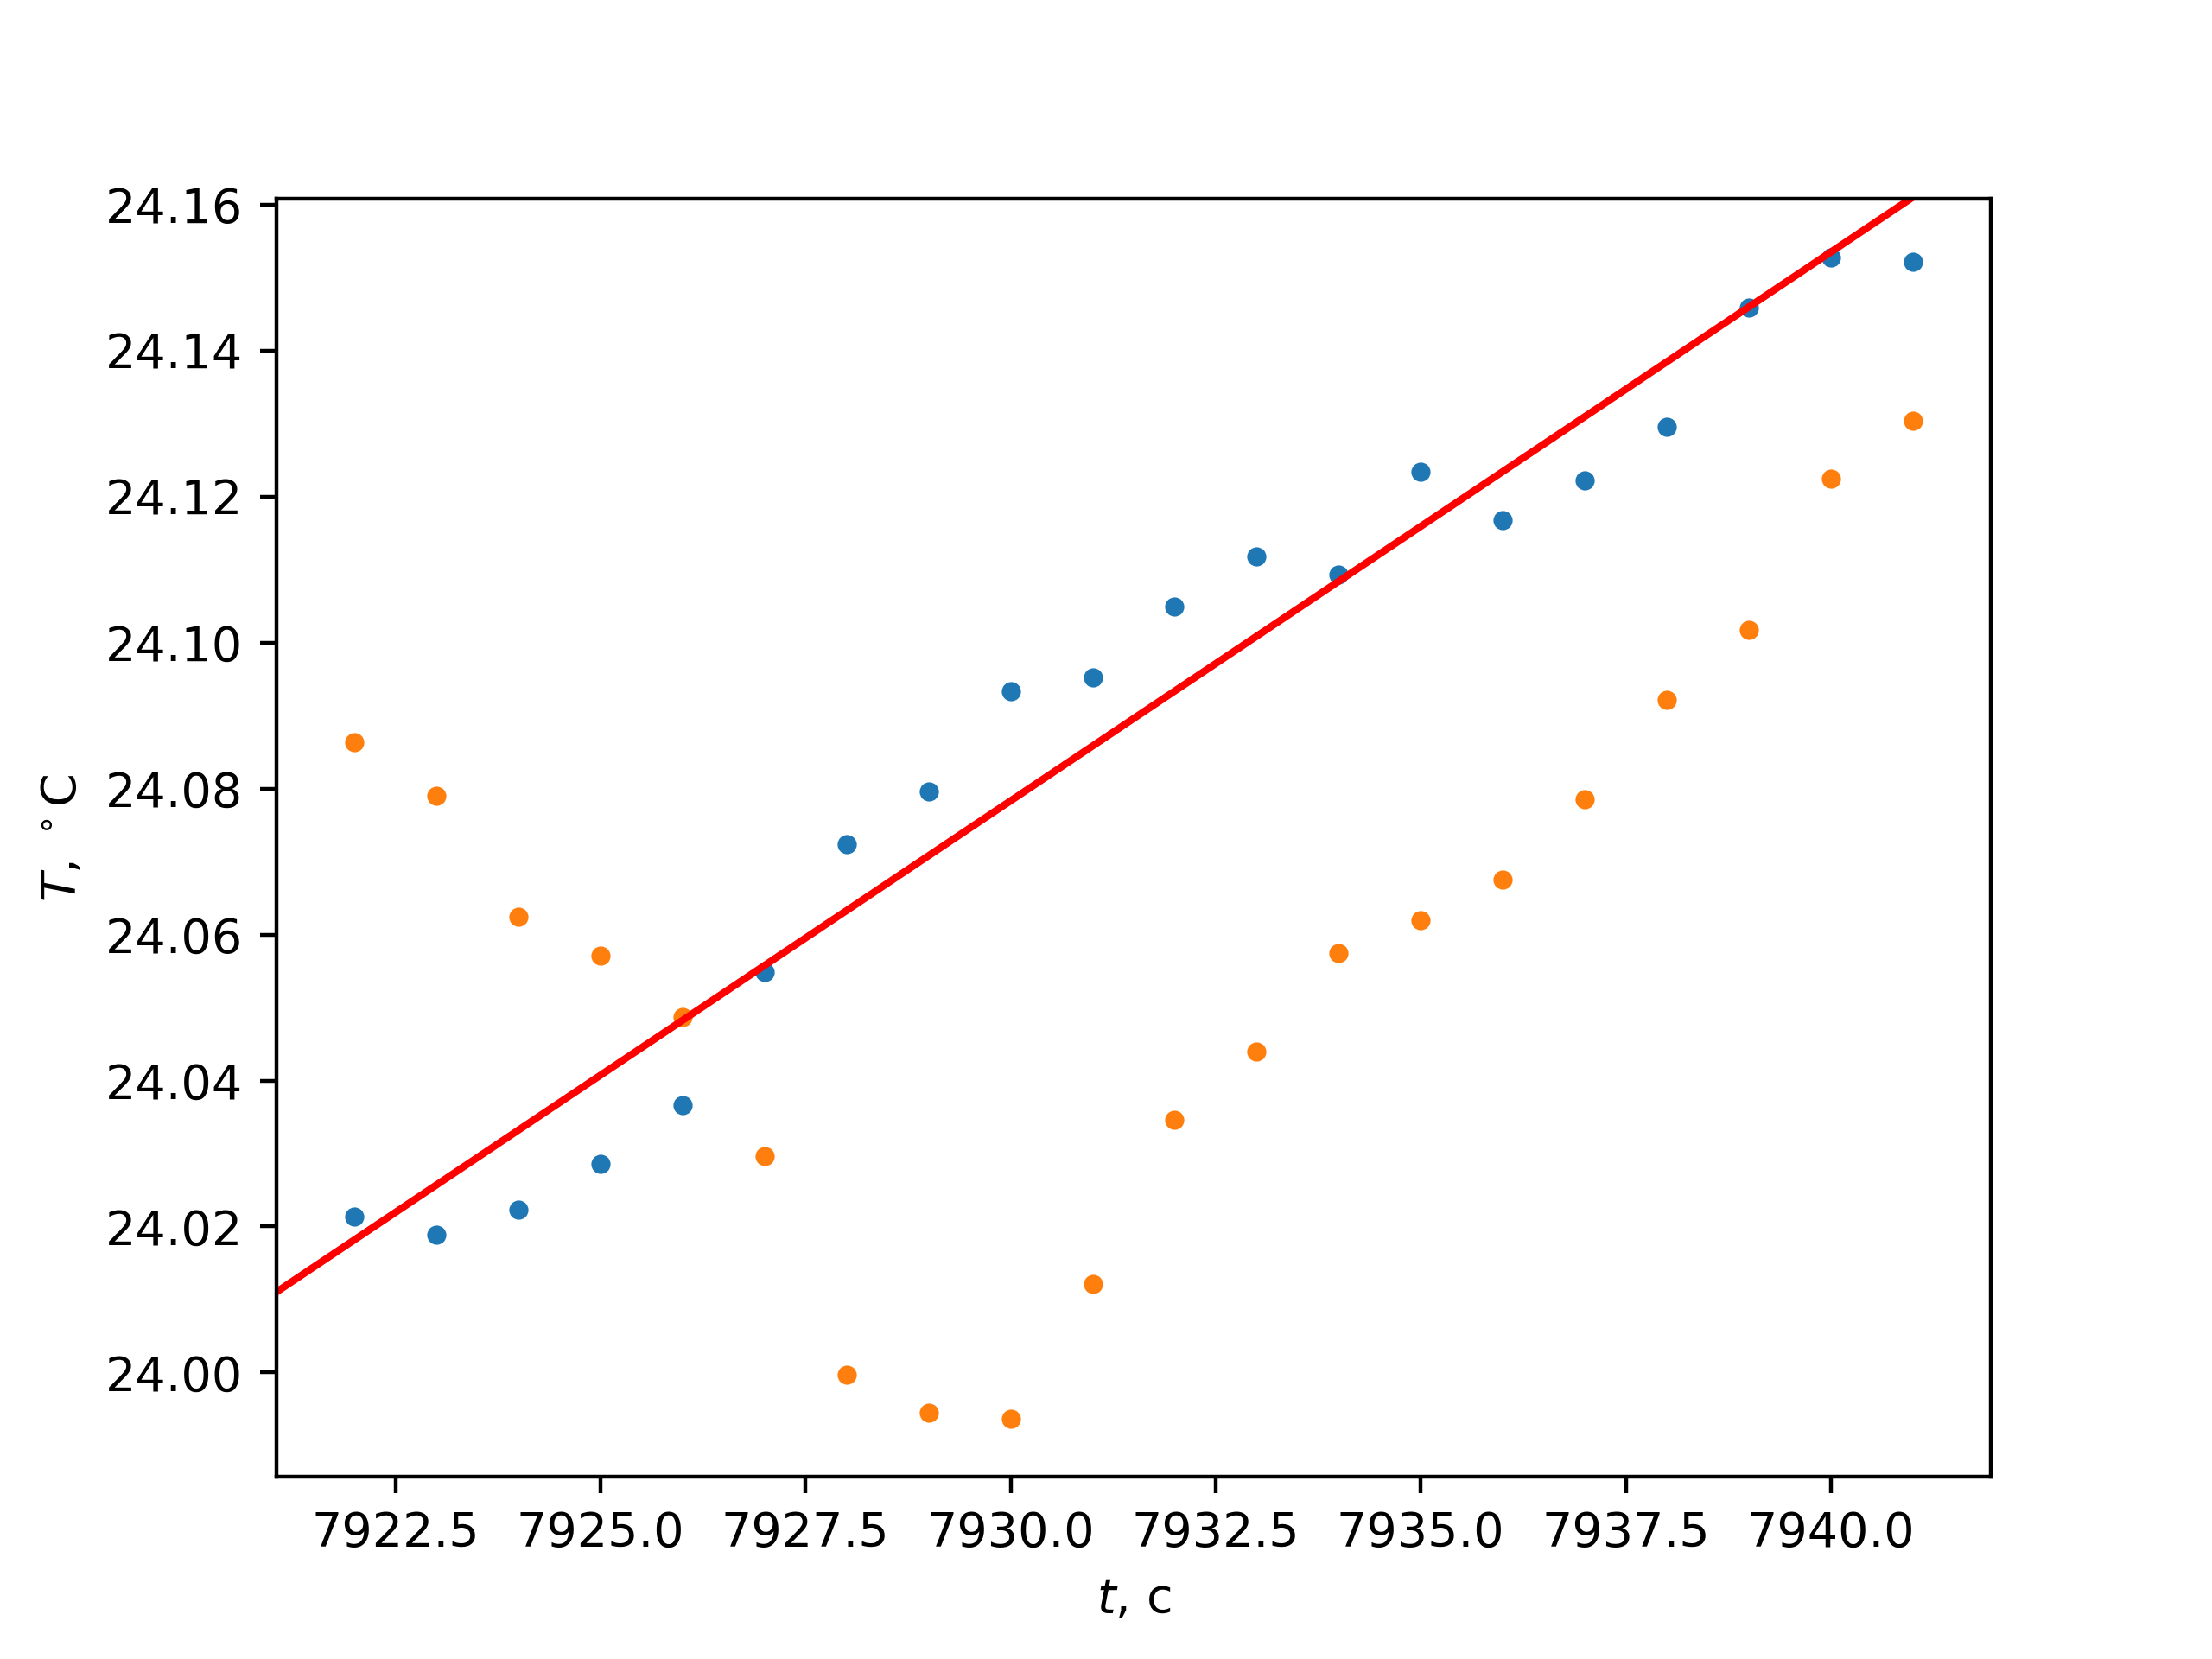
\includegraphics[width=0.6\linewidth]{img/7930.png}
        \caption{Касательная к кривой нагрева калориметра с алюминиевым конусом}
    \end{figure}

    В этом методе получилось большое отклонение от табличных значений и большие
    погрешности. Это связано с малым количеством экспериментальных точек и возможным
    различием температур вблизи калориметра и термометра, из-за чего мог возникнуть теплообмен.
\newpage~
\newpage
    \subsection{Дифференциальный метод в окрестности точек с одинаковой температурой}

    Вблизи точек с одинаковой температурой можно определить теплоемкость $C$:
    \[C=\frac{P}{A-B+A\frac{T_{\text{K}_1}-T_{\text{K}_2}}{T-T_{\text{K}_1}}}\]
    \[A=\left(\frac{dT}{dt}\right)_\text{heat}\]
    \[B=\left(\frac{dT}{dt}\right)_\text{cool}\]
    $T$~--- температура, вблизи которой строятся касательные, $T_{\text{K}_1}$~---
    комнатная температура в момент охлаждения, $T_{\text{K}_2}$~---
    комнатная температура в момент нагревания.

    Рассмотрим $T=29\,^\circ\text{C}$.

    Необходимо строить касательные в моменты времени:
    \begin{enumerate}
        \item $1955\,\text{с}$ и $2510\,\text{с}$ для пустого калориметра
        $$T_{\text{K}_1}=21{,}97\pm 0{,}05\,\text{К}$$
        $$T_{\text{K}_2}=22{,}11\pm 0{,}05\,\text{К}$$
        $$T=29{,}01\pm 0{,}05\,\text{К}$$
        $$A=0{,}0064\pm 0{,}0002\,\frac{\text{К}}{\text{с}}$$
        $$B=-0{,}0025\pm 0{,}0002\,\frac{\text{К}}{\text{с}}$$
        $$C=680\pm 20\,\frac{\text{Дж}}{\text{К}}$$
        \item $5195\,\text{с}$ и $6175\,\text{с}$ для калориметра с железом
        $$T_{\text{K}_1}=22{,}70\pm 0{,}05\,\text{К}$$
        $$T_{\text{K}_2}=23{,}00\pm 0{,}05\,\text{К}$$
        $$T=29{,}00\pm 0{,}05\,\text{К}$$
        $$A_\text{Fe}=0{,}0042\pm 0{,}0002\,\frac{\text{К}}{\text{с}}$$
        $$B_\text{Fe}=-0{,}0011\pm 0{,}0002\,\frac{\text{К}}{\text{с}}$$
        $$C_\text{Fe}=1180\pm 60\,\frac{\text{Дж}}{\text{К}}$$
        $$c_\text{Fe}=610\pm80\,\frac{\text{Дж}}{\text{кг}\cdot\text{К}}$$
        \item $8753\,\text{с}$ и $9988\,\text{с}$ для калориметра с алюминием
        $$T_{\text{K}_1}=24{,}26\pm 0{,}05\,\text{К}$$
        $$T_{\text{K}_2}=24{,}33\pm 0{,}05\,\text{К}$$
        $$T=29{,}01\pm 0{,}05\,\text{К}$$
        $$A_\text{Al}=0{,}0055\pm 0{,}0002\,\frac{\text{К}}{\text{с}}$$
        $$B_\text{Al}=-0{,}0046\pm 0{,}0004\,\frac{\text{К}}{\text{с}}$$
        $$C_\text{Al}=1010\pm 40\,\frac{\text{Дж}}{\text{К}}$$
        $$c_\text{Al}=1150\pm40\,\frac{\text{Дж}}{\text{кг}\cdot\text{К}}$$
    \end{enumerate}

    Значения ояпть сильно отличаются от табличных из-за неточности
    построения касательных (аналогично предыдущему методу).

    \begin{figure}[ht!]
        \centering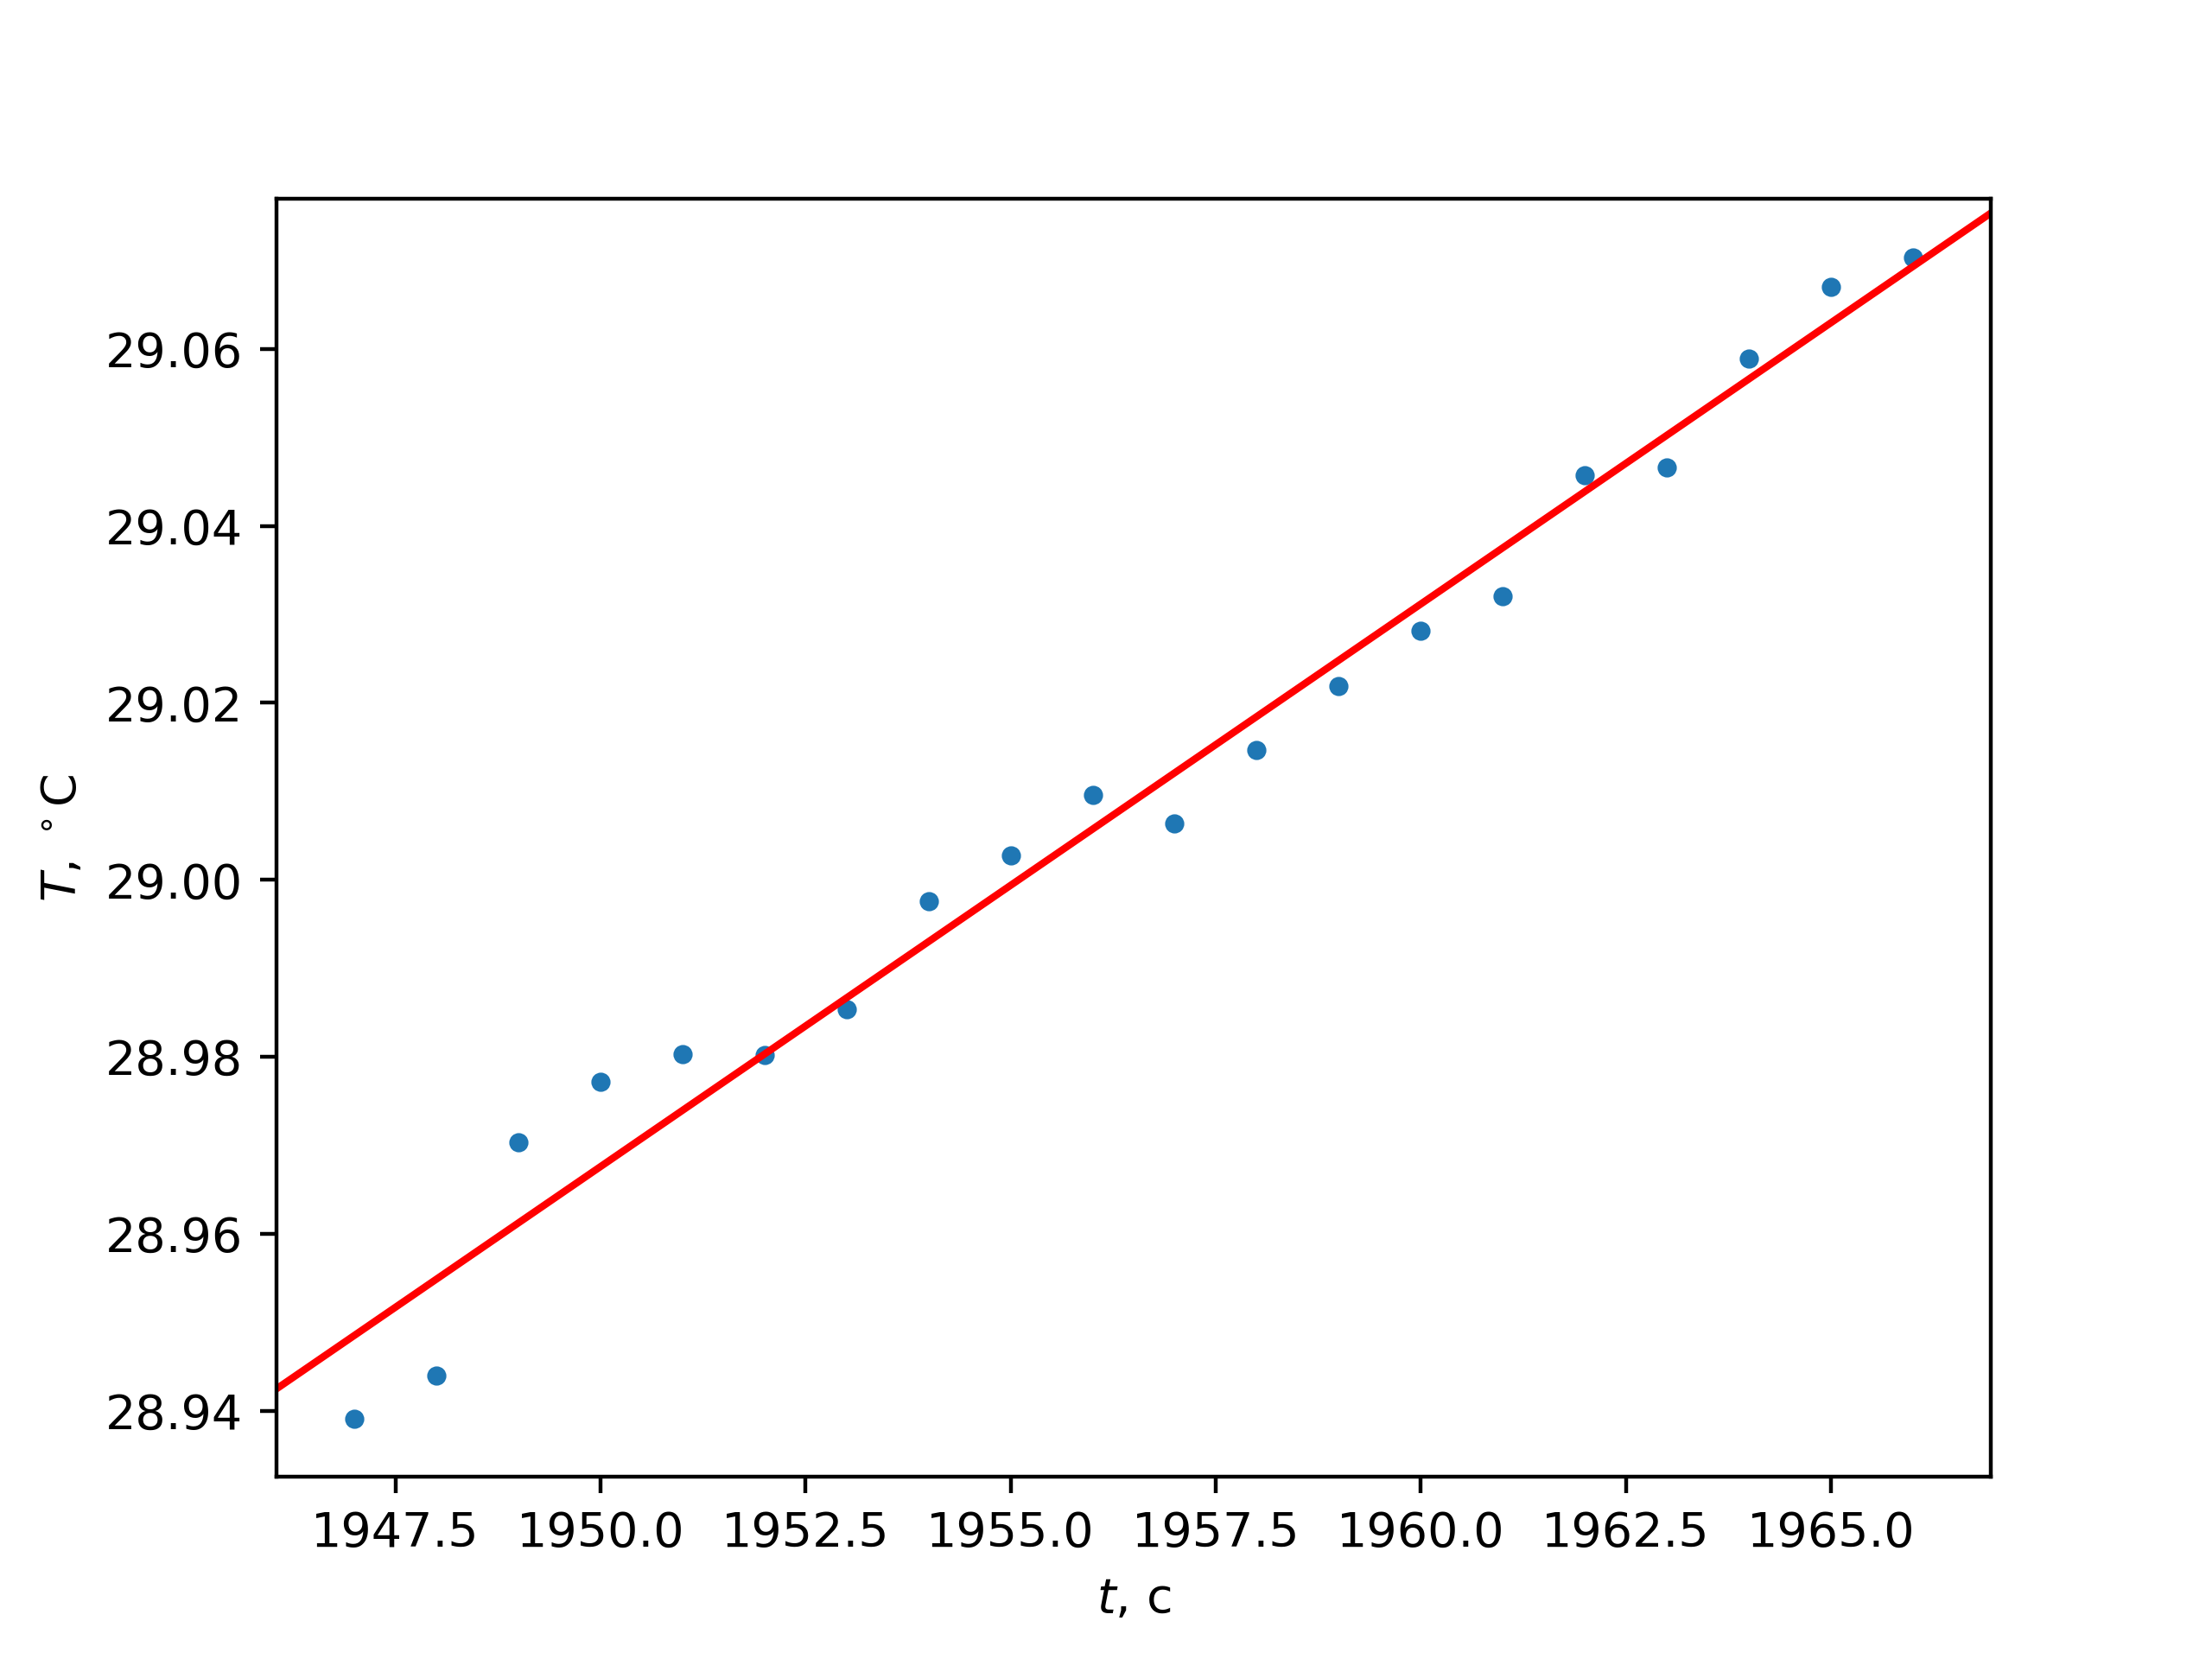
\includegraphics[width=0.6\linewidth]{img/1955.png}
        \caption{$t=1955\,\text{с}$}
    \end{figure}
    \begin{figure}[ht!]
        \centering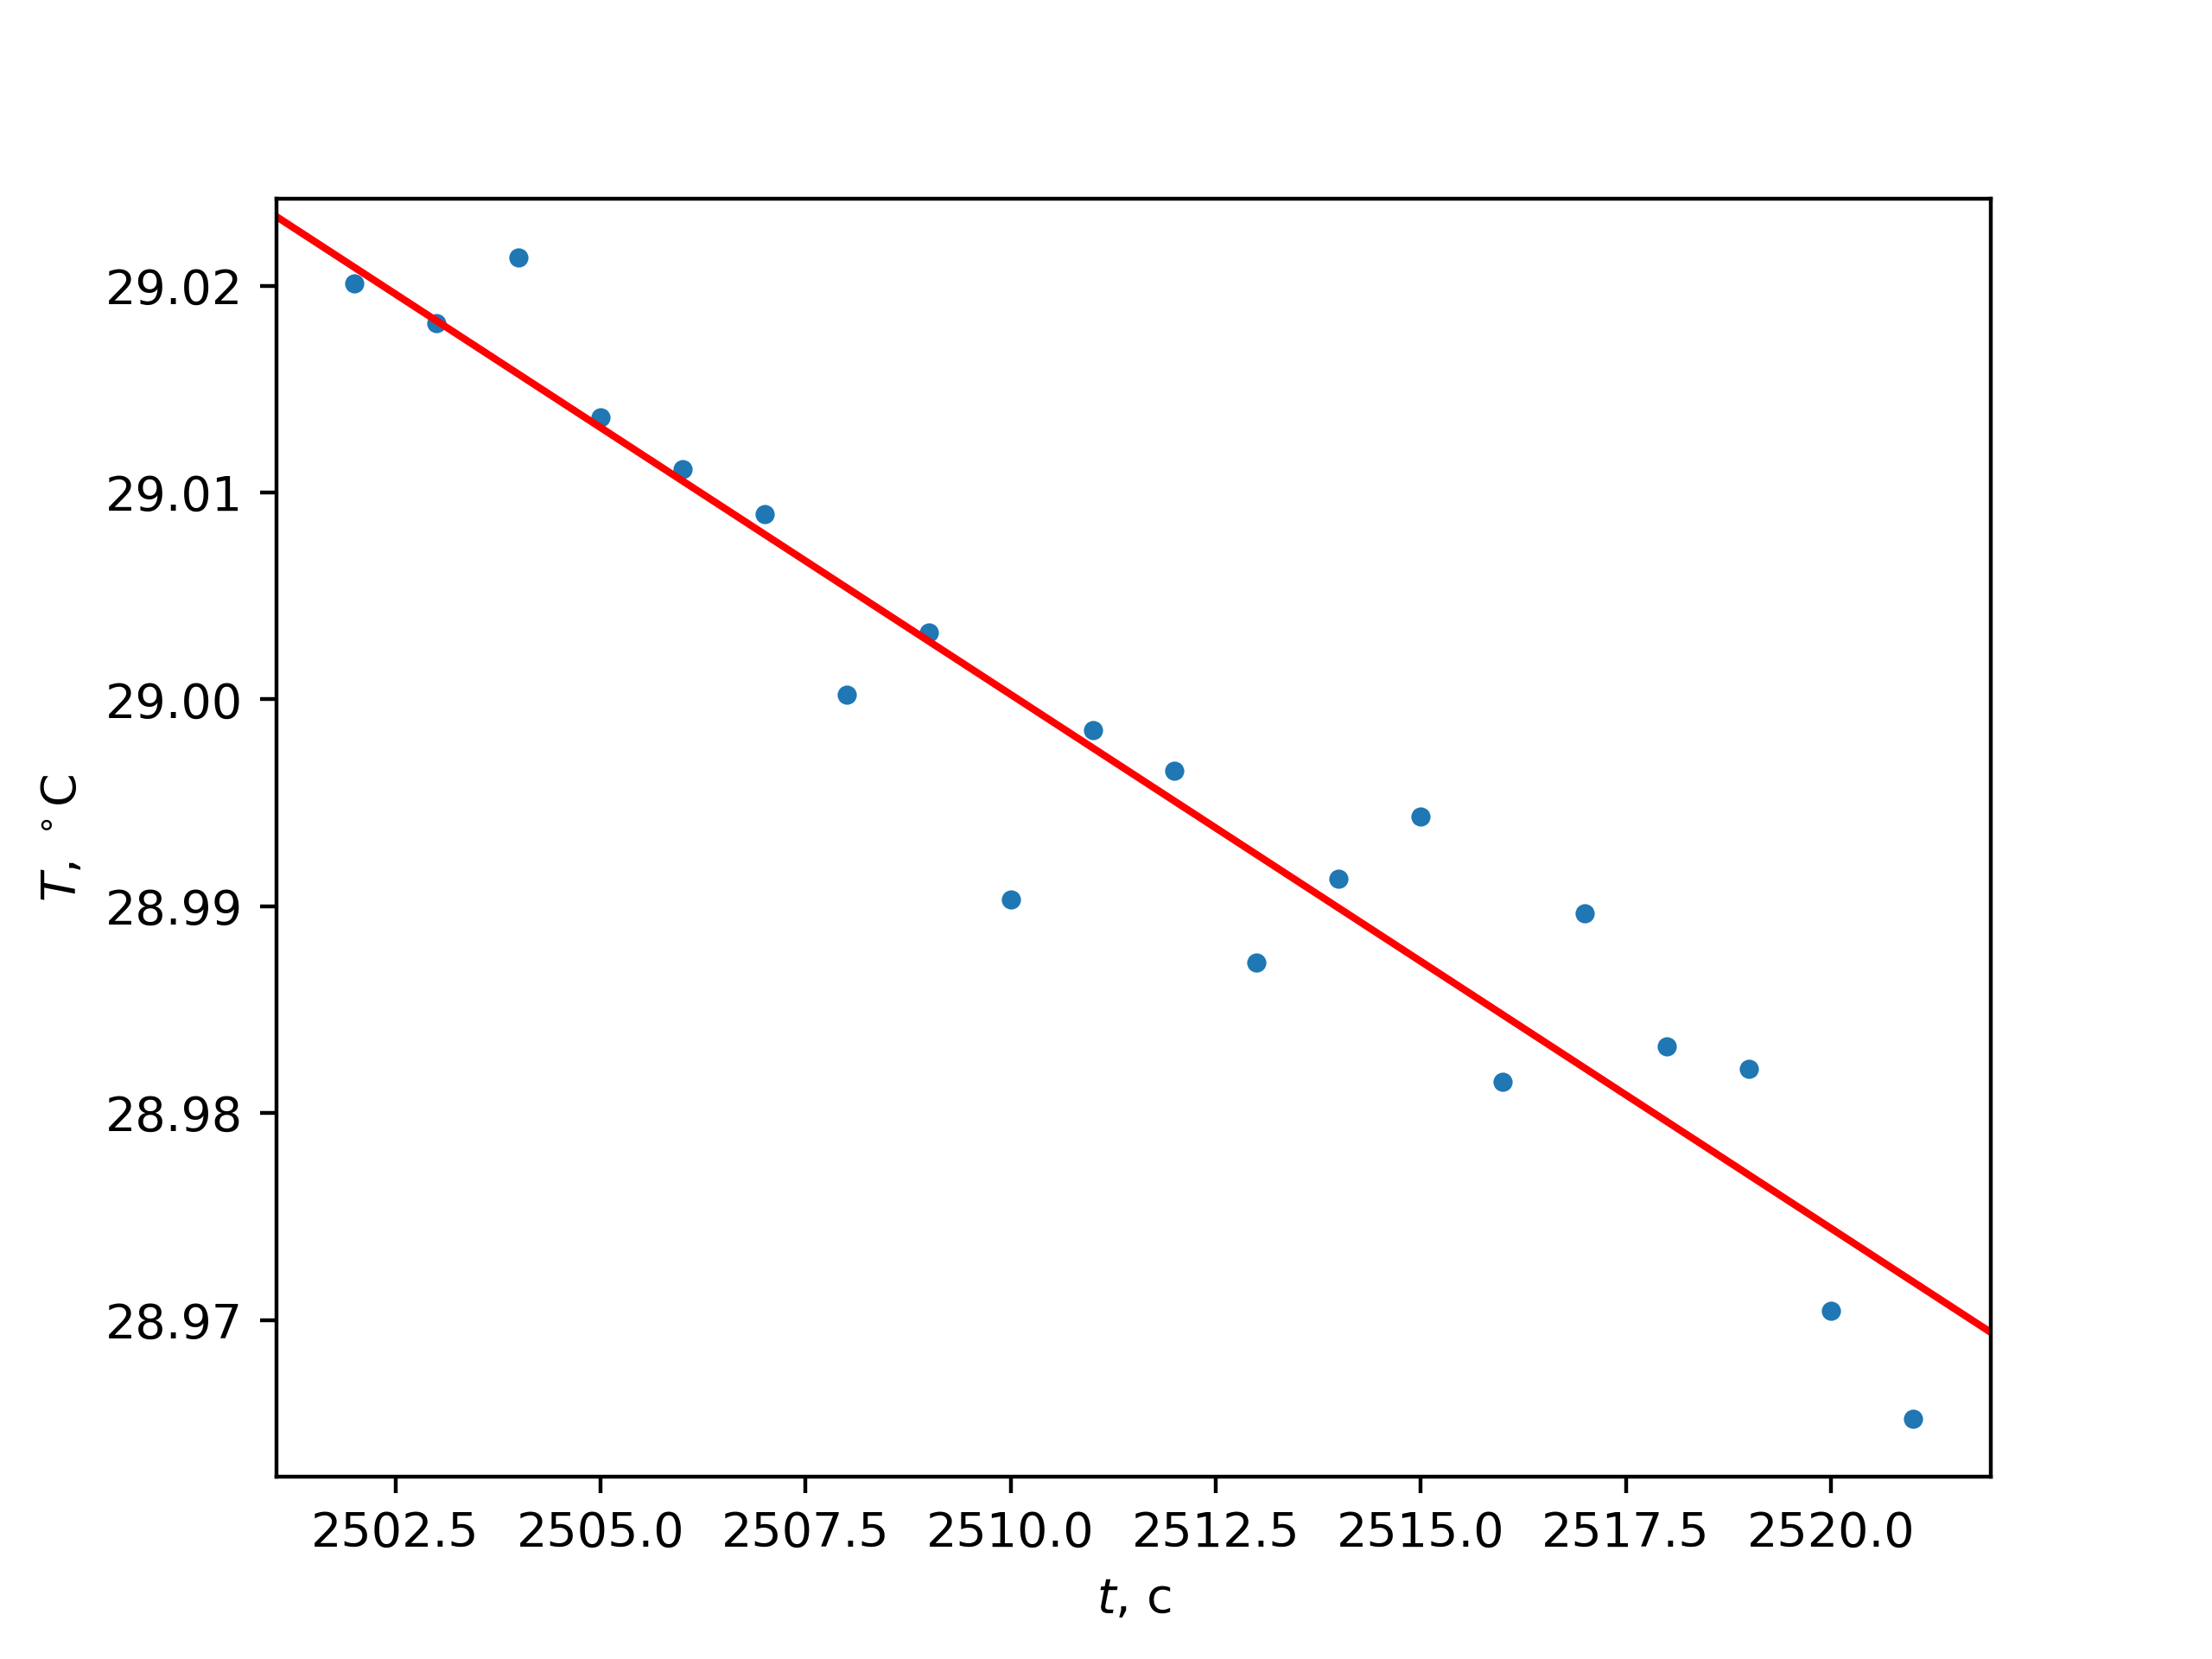
\includegraphics[width=0.6\linewidth]{img/2510.png}
        \caption{$t=2510\,\text{с}$}
    \end{figure}
    \begin{figure}[ht!]
        \centering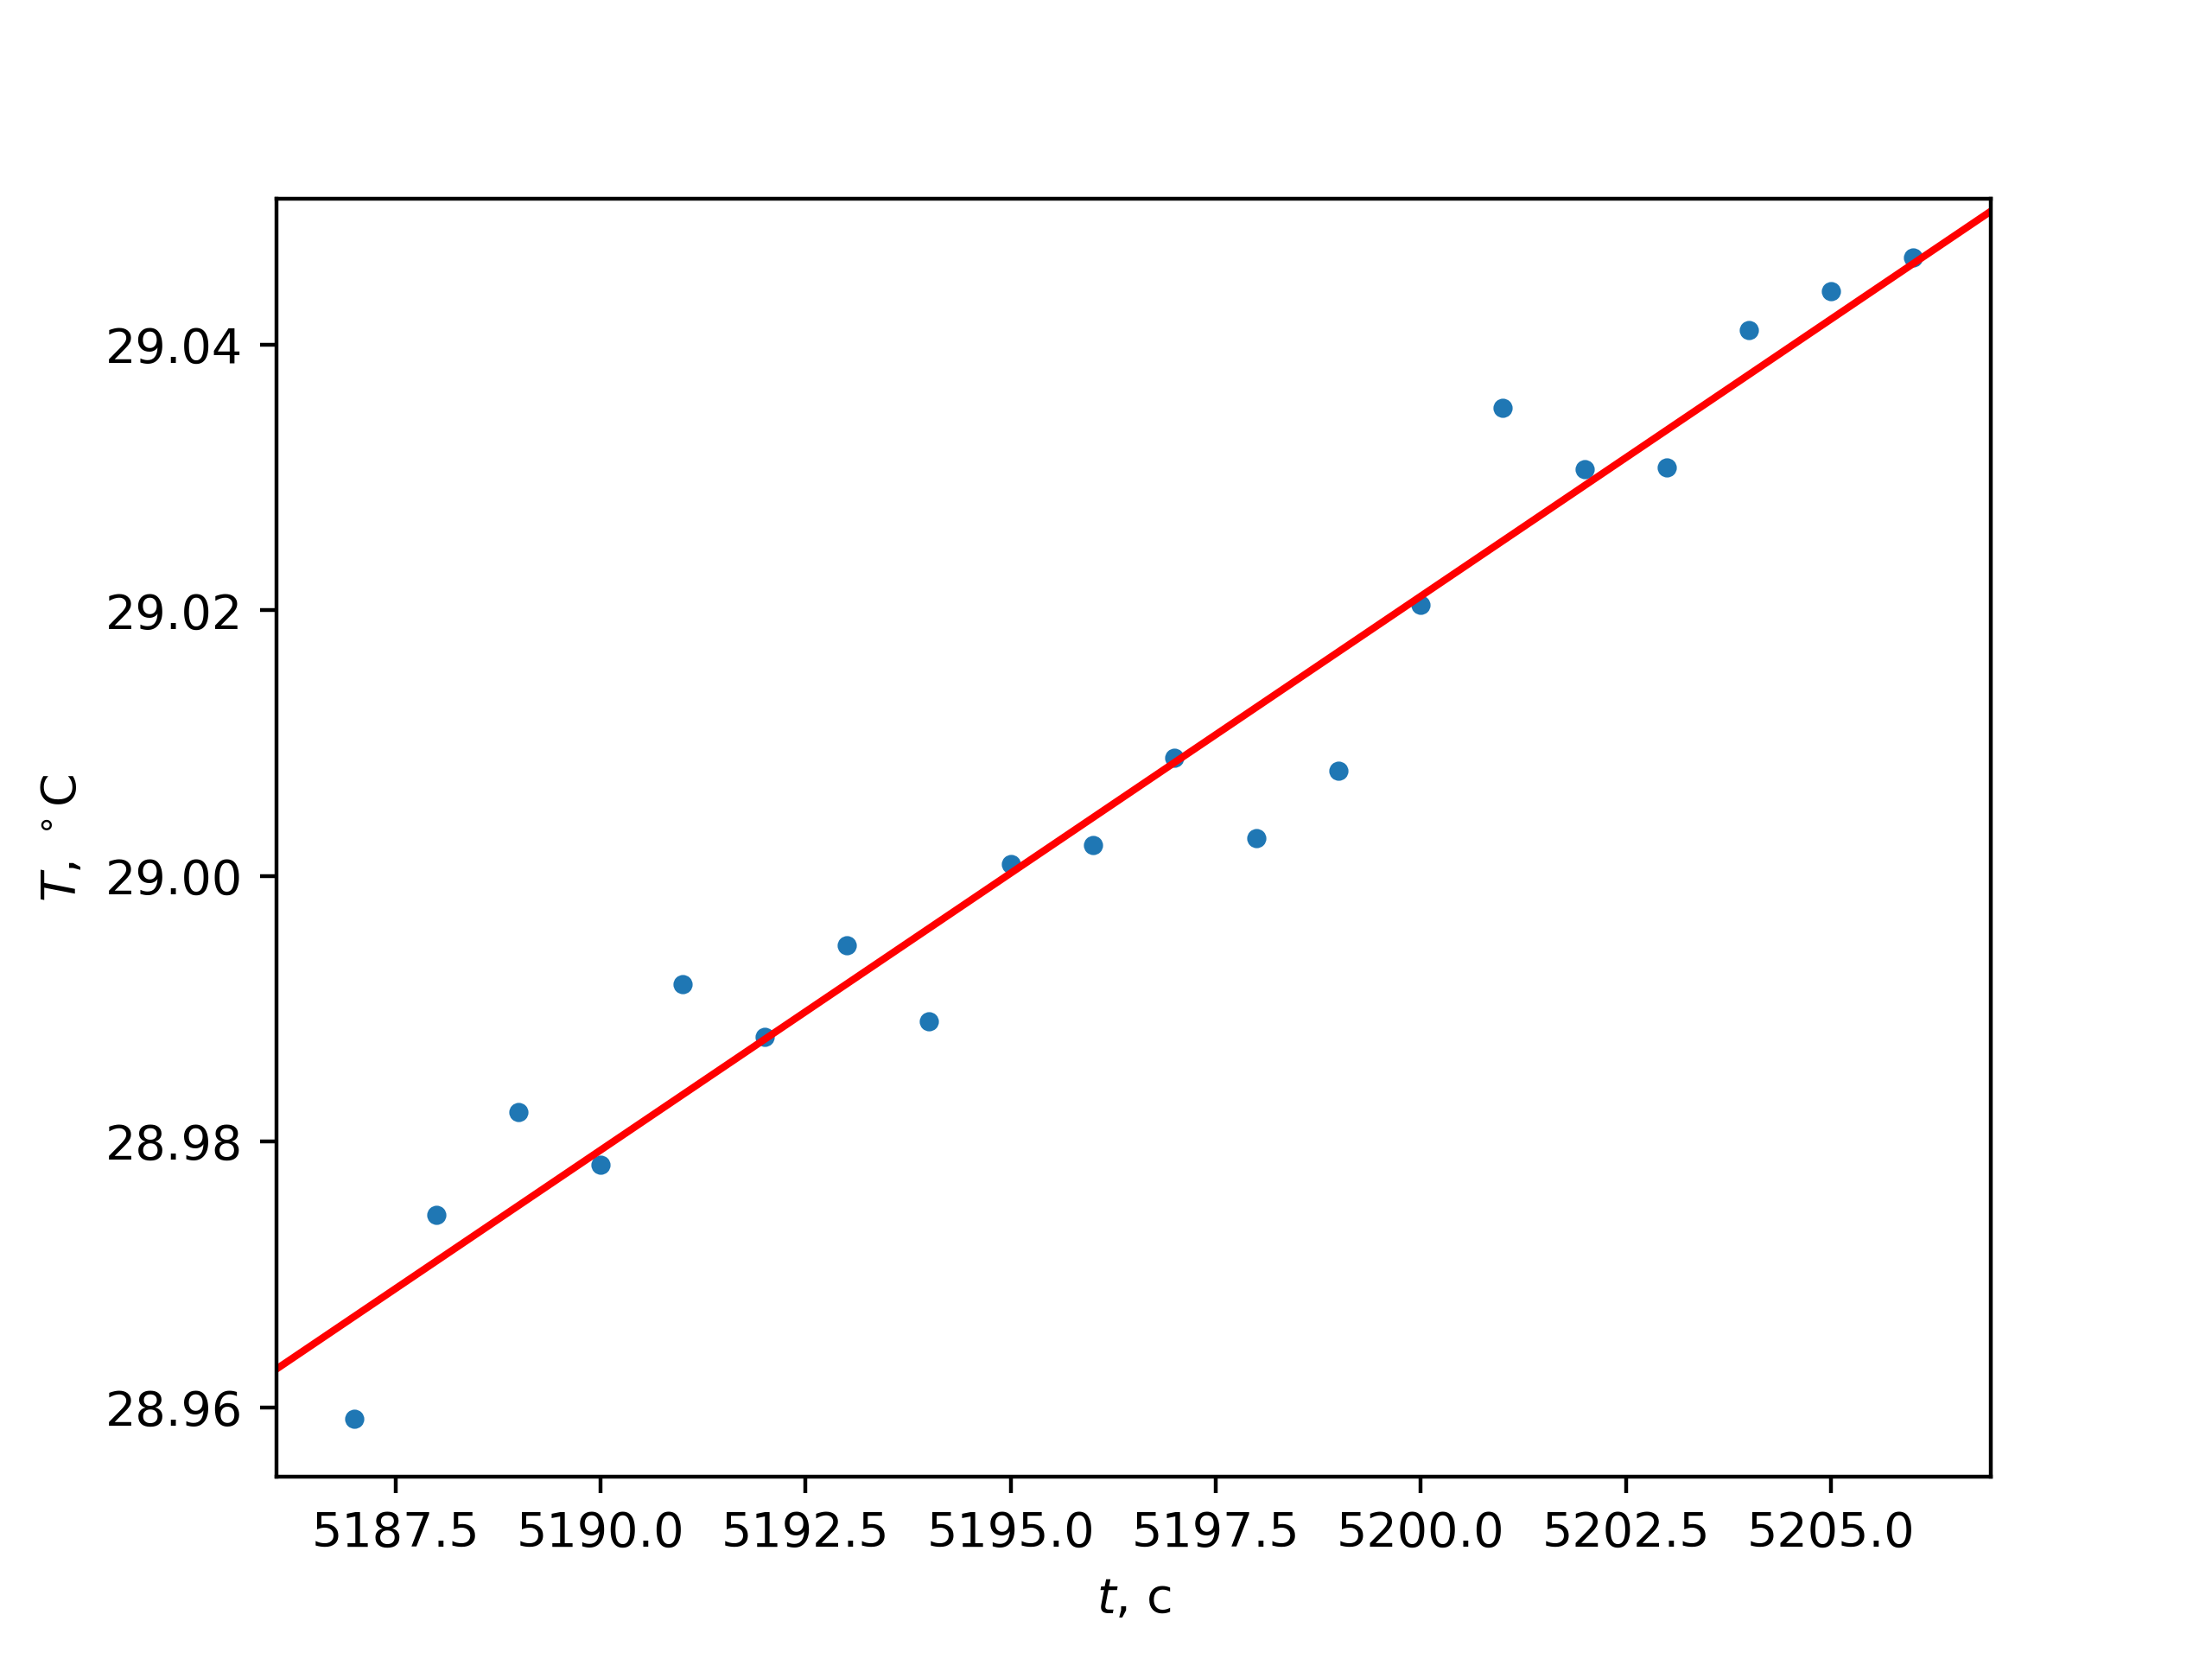
\includegraphics[width=0.6\linewidth]{img/5195.png}
        \caption{$t=5195\,\text{с}$}
    \end{figure}
    \begin{figure}[ht!]
        \centering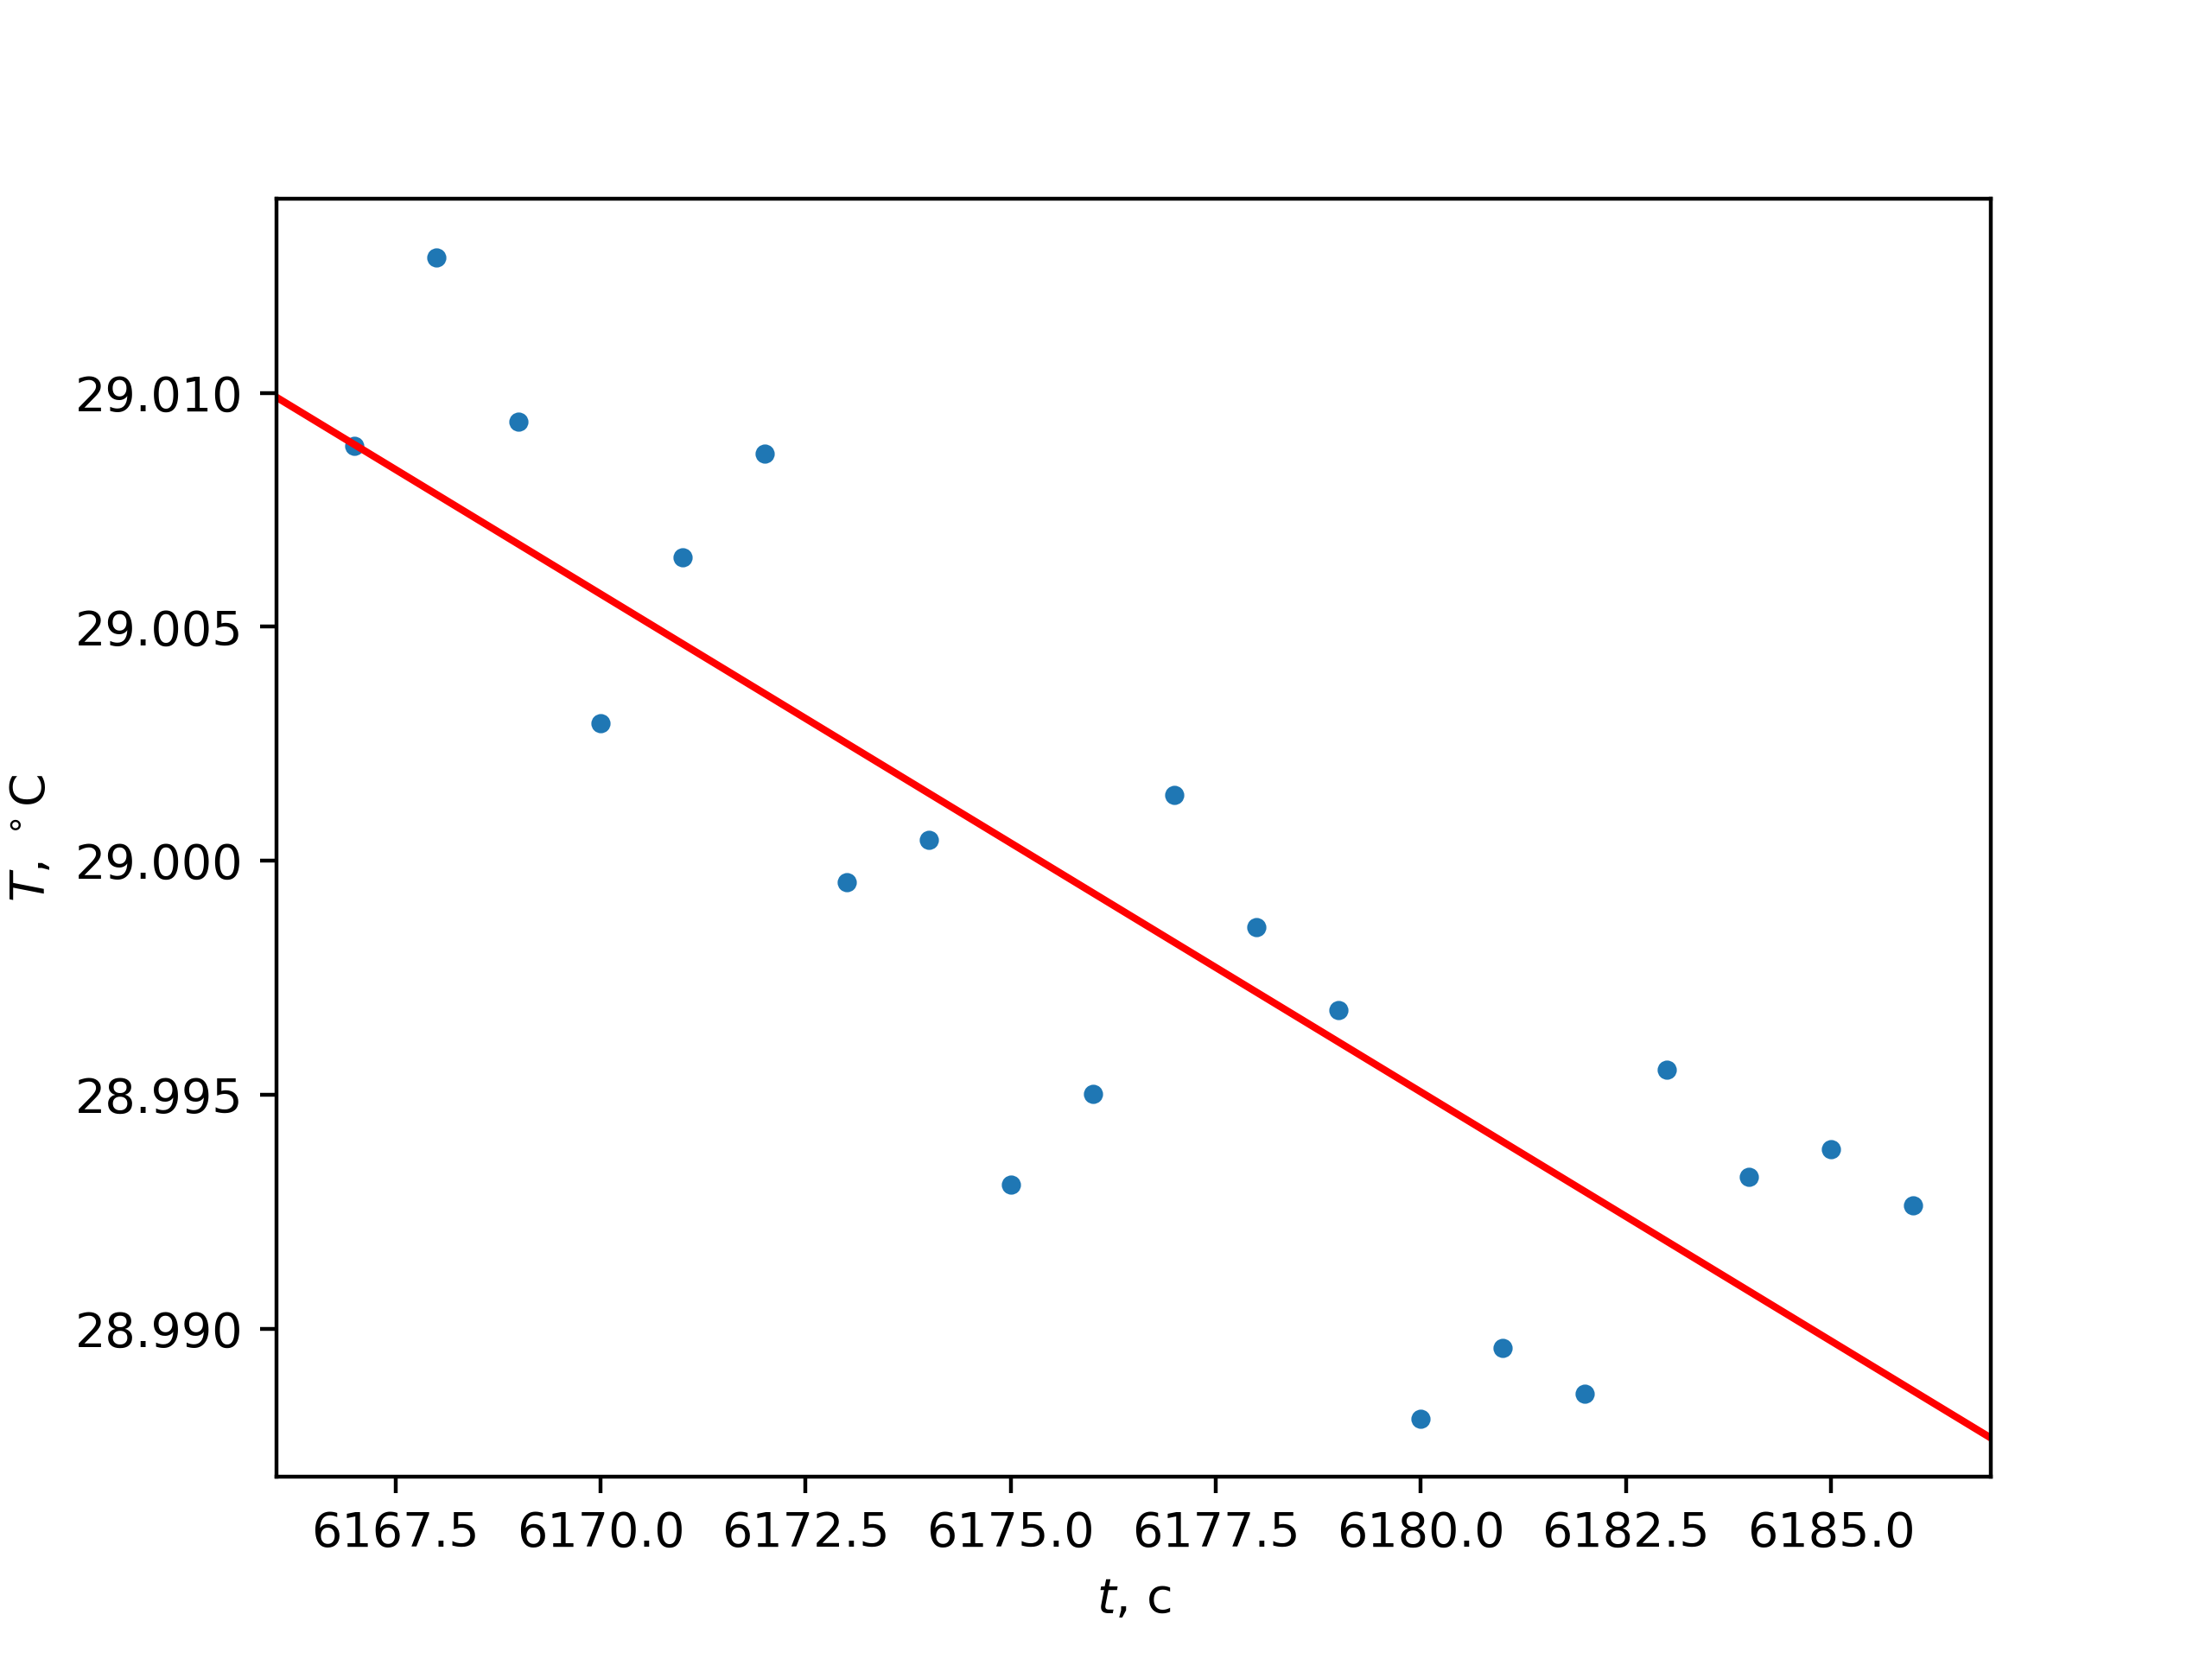
\includegraphics[width=0.6\linewidth]{img/6175.png}
        \caption{$t=6175\,\text{с}$}
    \end{figure}
    \begin{figure}[ht!]
        \centering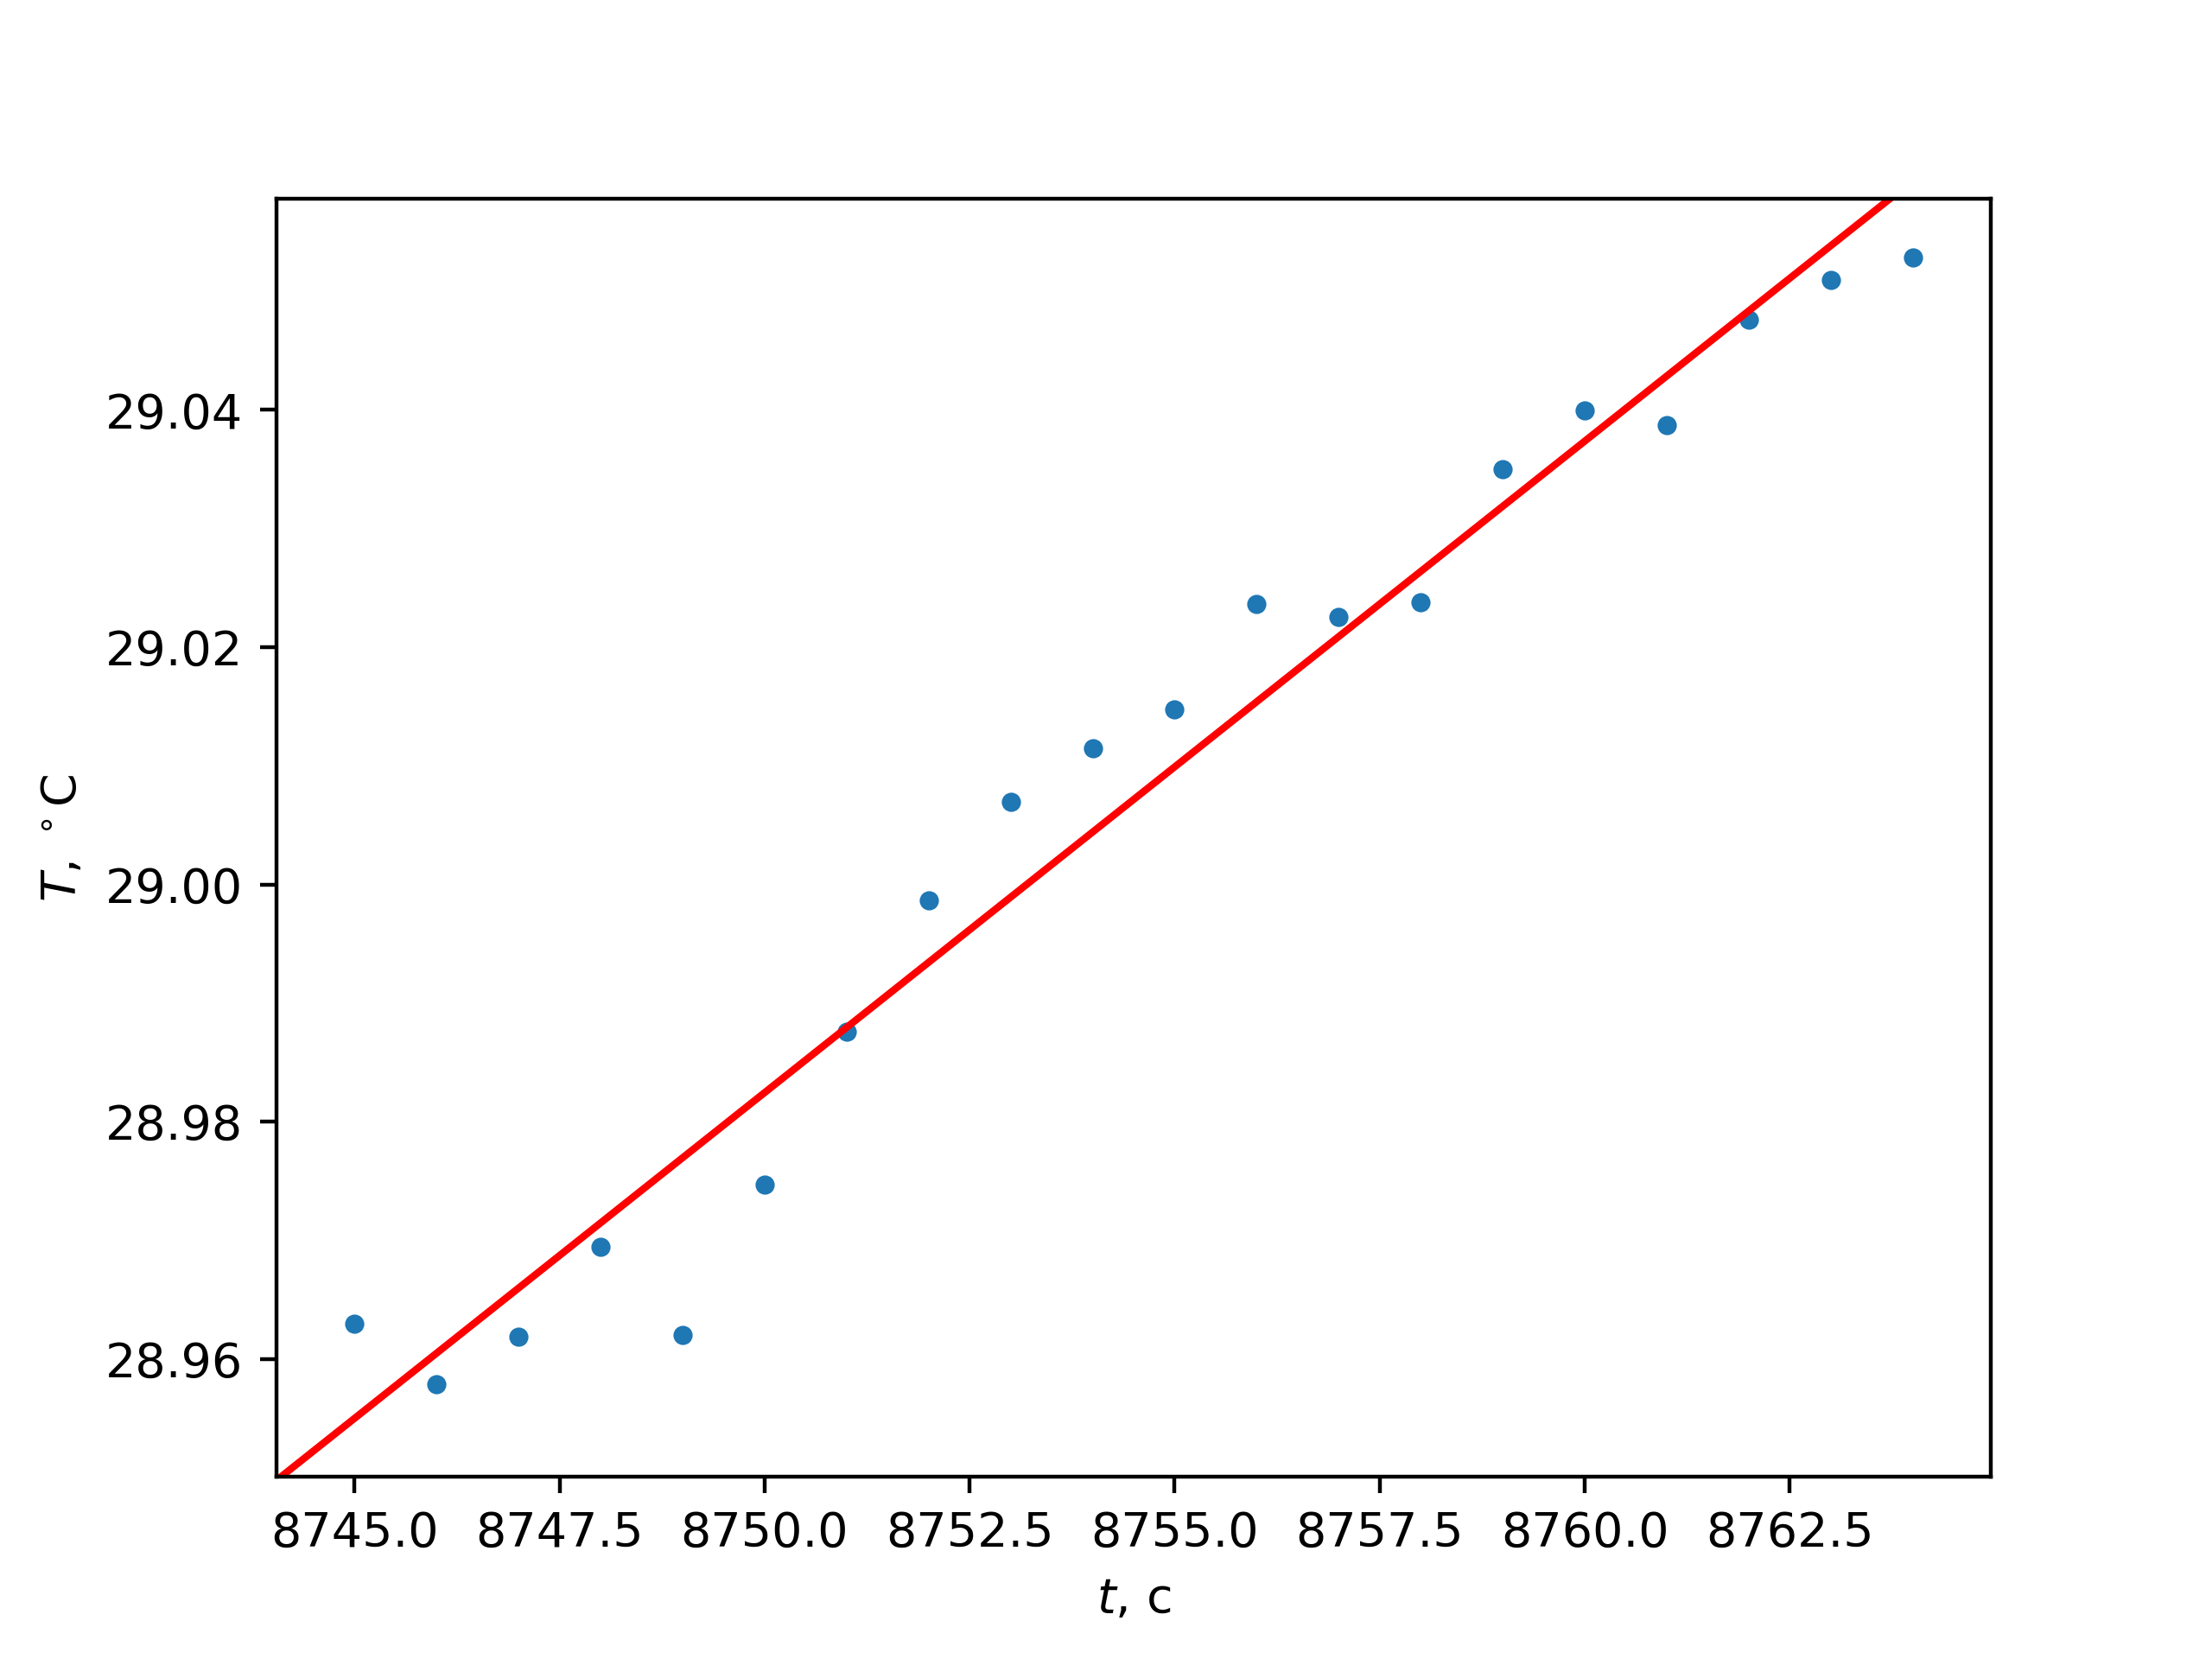
\includegraphics[width=0.6\linewidth]{img/8753.png}
        \caption{$t=8753\,\text{с}$}
    \end{figure}
    \begin{figure}[ht!]
        \centering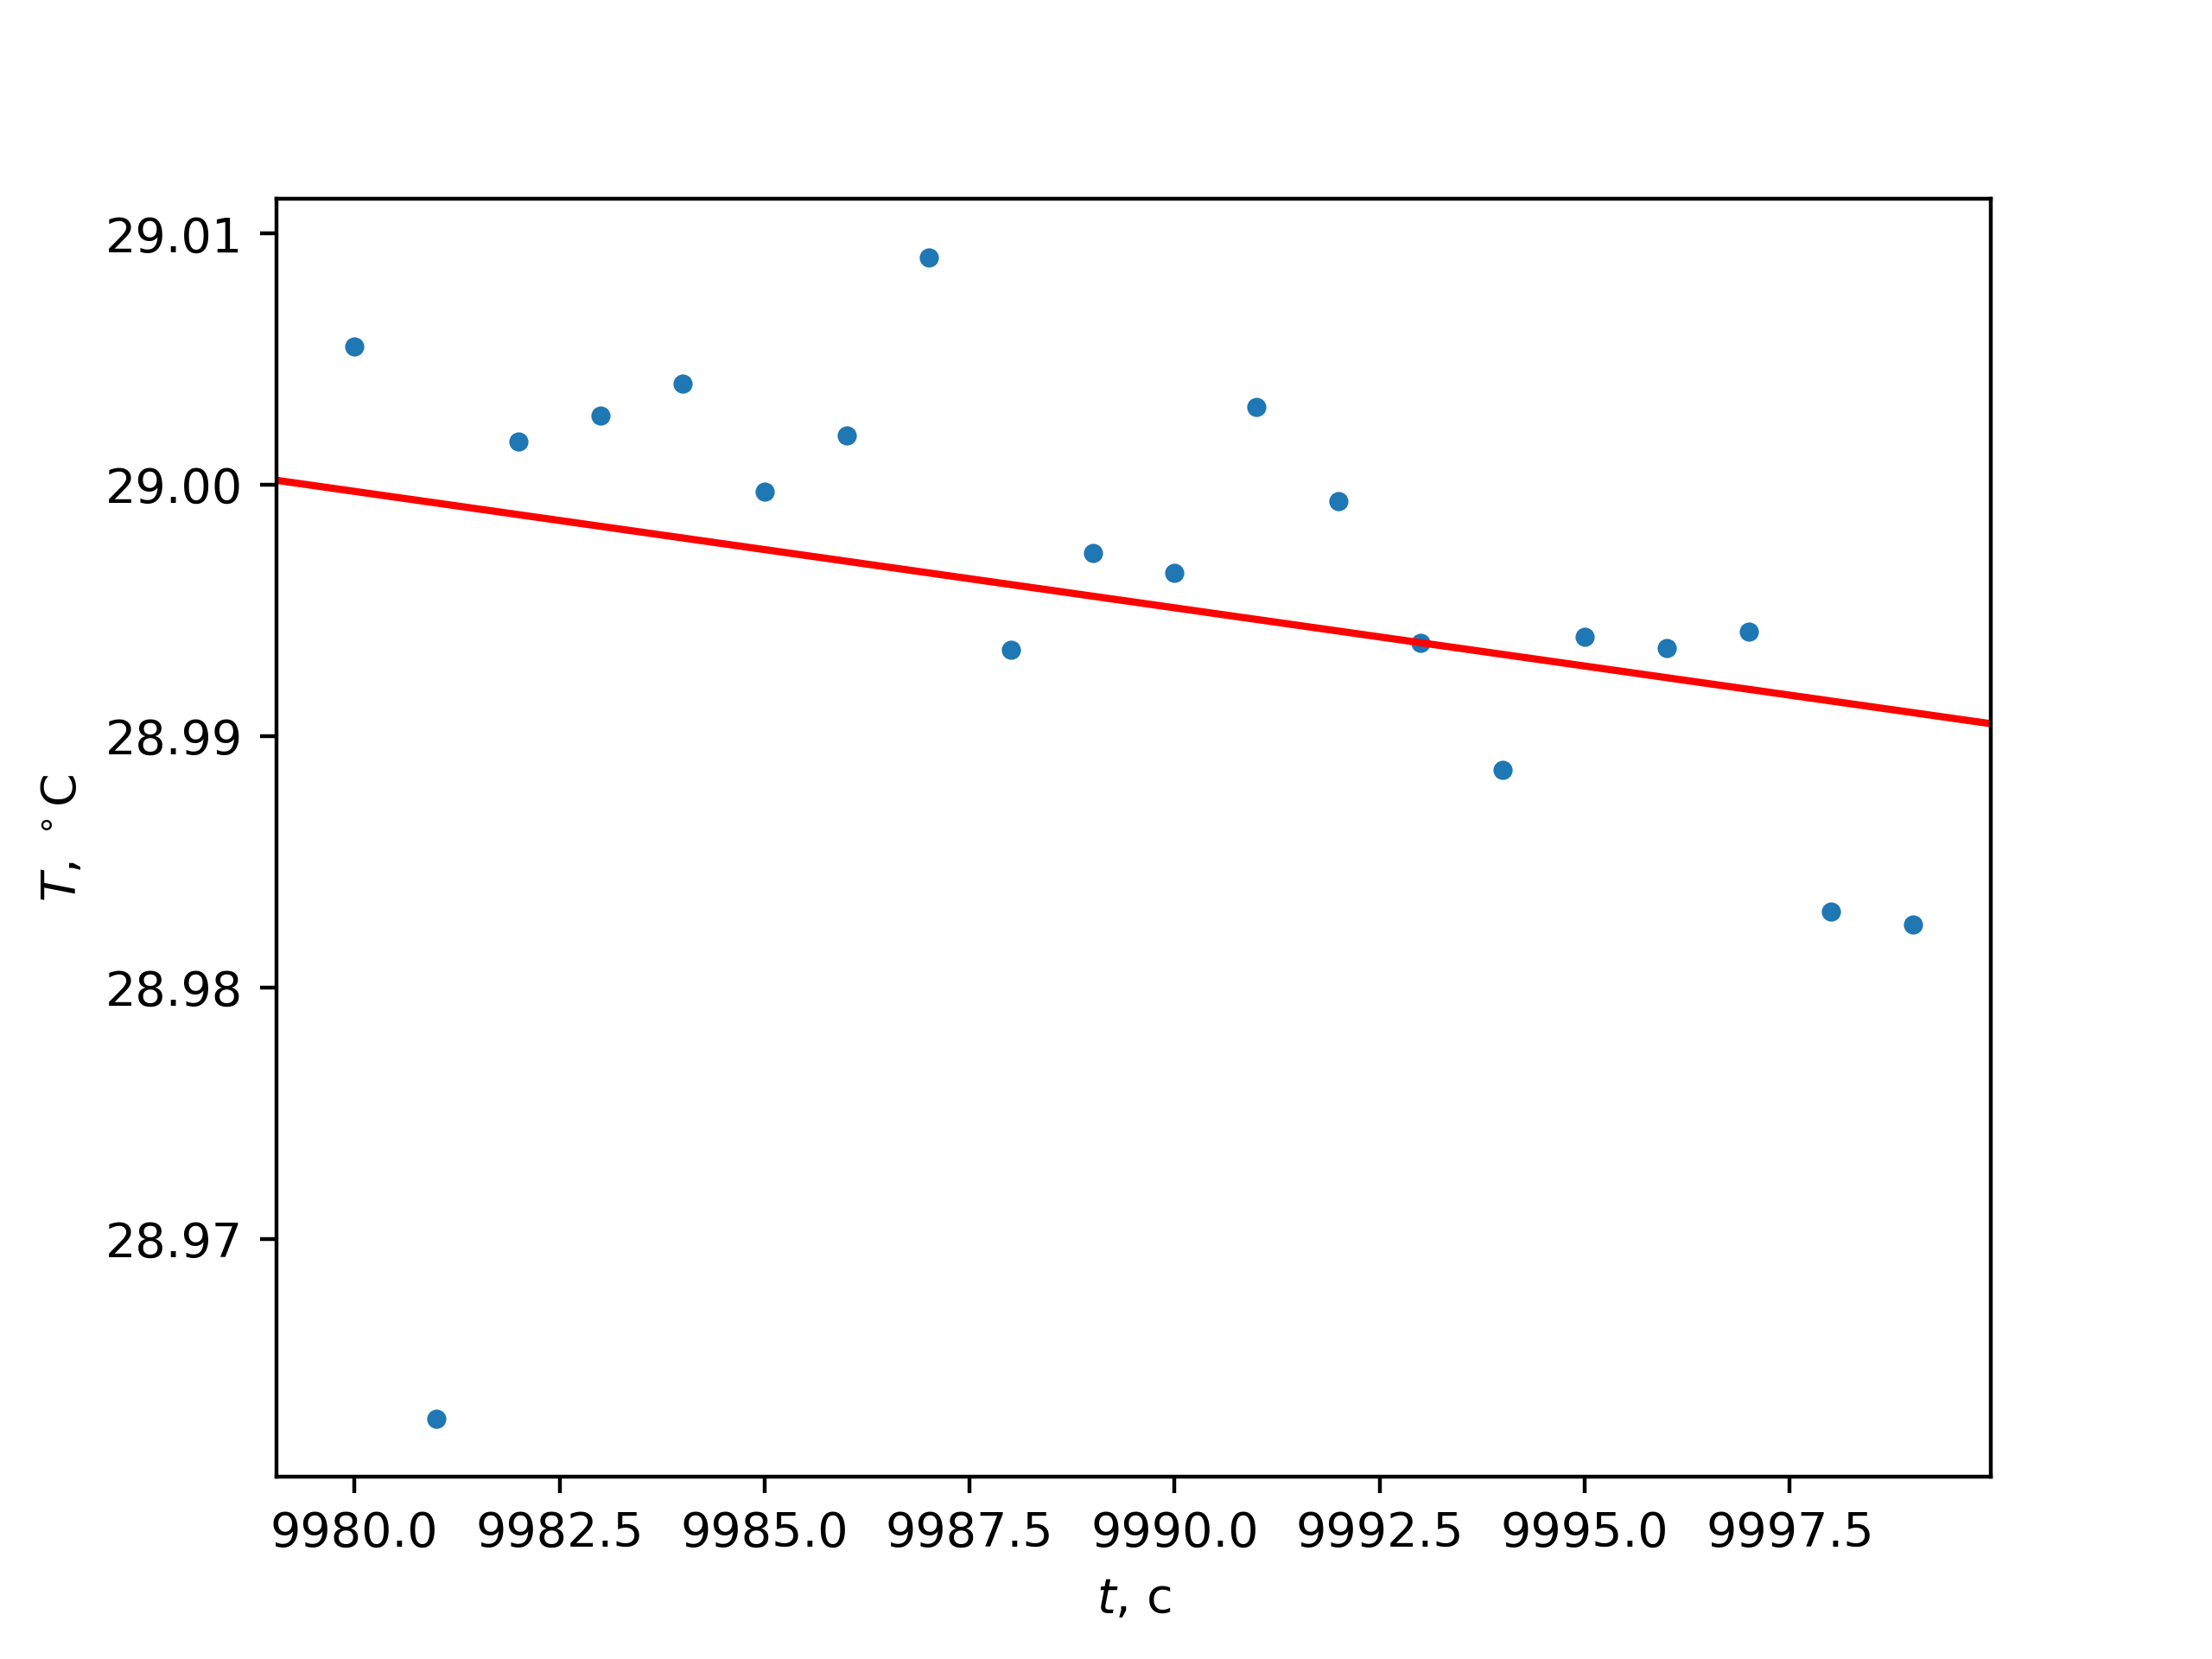
\includegraphics[width=0.6\linewidth]{img/9988.png}
        \caption{$t=9988\,\text{с}$}
    \end{figure}

\end{document}